\documentclass[usegeometry=true]{scrartcl}
\usepackage[ngerman]{babel}
\usepackage[T1]{fontenc}
\usepackage{lmodern}
\usepackage[utf8]{inputenc}
\usepackage{hyperref}
\usepackage{amssymb}
\usepackage{graphicx}
\usepackage{wrapfig}
% Dimensionen bitte nicht ändern. 
\usepackage[left=2cm, right=2cm, top=2cm, bottom=2cm, bindingoffset=1cm, includeheadfoot]{geometry}
%Zeilenabstand bitte nicht ändern
\usepackage[onehalfspacing]{setspace}

\usepackage[backend=biber,style=numeric,]{biblatex}\addbibresource{literatur.bib}

\begin{document}
\pagenumbering{gobble}
% ----------------------------------------------------------------------------
\subject{Projektbericht zum Modul Information Retrieval und Visualisierung Sommersemester 2022}
\title{Marktanalyse des Videospielemarktes}
\subtitle{Analyse und Visualsierung der Verkaufszahlen der Videospiele auf der Platform XBoxOne}
\author{Lena Arloth\\
        Matrikelnummer: 217207784}% obligatorisch
%\date{10.9.2022}

\dedication{\normalsize\vfill\hrule\vspace{10pt}
            Link zum GitHub-Repository:\\
            \url{https://github.com/Lena-Ar/Info-Vis}\\
            Letzter Commit: \\
            () \\
            \vspace{10pt}
            Link zur öffentlich zugänglichen Website (GitHub-Pages):\\
            \url{https://lena-ar.github.io/Info-Vis/}
            }

\maketitle% verwendet die zuvor gemachte Angaben zur Gestaltung eines Titels
% ----------------------------------------------------------------------------
\newpage
%Inhaltsverzeichnis:
\tableofcontents
% ----------------------------------------------------------------------------
% Gliederung und Text:
\newpage
\pagenumbering{arabic}
\section{Einleitung}
Der weltweite, plattformübergreifende Videospielmarkt besaß im Jahr 2021 mit ein Volumen von 156,17 Milliarden Euro 
und wird 2022 voraussichtlich auf 176,13 Milliarden Euro steigen.\cite{Statista.2022b}
Entsprechend viel Geld und Potenzial durch Wachstum verbirgt sich in ihm.
Gleichzeitig bedarf es für die Entwicklung neuer Videospiele hohe Investitionen seitens der Entwicklerstudios und Verleger, folgend Publisher genannt, 
die erst nach einer gewissen Sicherheit durch Analyse des Marktes getroffen werden sollten.
Zur Findung von Prognosen und Tendenzen für die Zukunft, braucht es Erkenntnisse aus vergangenen Daten.
Eine Möglichkeit hierzu ist die Analyse der totalen Verkaufszahlen der Videospieltitel aufgeschlüsselt nach Genre weltweit.

Entscheidern innerhalb der Publisher fehlt jedoch ohne Analysen das Wissen, in welche Videospieltitel in welchem Genre und mit welcher Regionsausrichtung sie künftig investieren sollten, 
um das Potenzial des großen, wachsenden Videospielmarktes gewinnbringend zu nutzen.
Investition bezieht sich zunächst nicht zwingend auf konkrete Entscheidungen für die Auftragsvergabe neuer Titel, 
sondern vor allem auf die Veranlassung detaillierter, umfassender Marktstudien, auf deren Basis eine fundierte endgültige Entscheidung getroffen werden kann.
Zur Lösung dieser Problemstellung ergibt sich eine durchzuführende grobe Marktanalyse der Verkaufszahlen einer Plattform in der Videospielindustrie aus Sicht der Publisher.
Sie fungiert als Grundlage und Unterstützung weiterer Entscheidungen und Investitionen.

Die Relevanz ergibt sich aus zuvor Beschriebenem und der Notwendigkeit von Marktanalysen als Voraussetzung für unternehmerische Entscheidungen, Chancen und Risiken sowie Potenzialen.\cite{Fleig.2020}
Für Publisher ist es bedeutend zu erfahren, was und in welchem Genre künftig mit guten Verkaufschancen entwickelt werden soll.
Weiterhin ist es relevant, mittels einer Marktanalyse zu erfahren, wie das Unternehmen selbst im Markt aufgestellt ist und was die Konkurrenz bietet. 
Es entsprechend wichtig, die vorhandenen Daten der kumulierten Verkaufszahlen aufgeschlüsselt nach Genre und in diesem nach Regionen auf Zusammenhänge und Auffälligkeiten zu untersuchen. 
Für ein erleichtertes Verständnis sowie das Aufdecken dieser sind Techniken aus dem Bereich der Visual Analytics von kritischer Relevanz.

Es leitet sich folgende Fragestellung ab, die es mittels oben genannter, grobgranularer und durch Visualisierungstechniken unterstützer Marktanalyse zu beantworten gilt:\\
In welches Genre und mit welchem Fokus auf die Regionen der Welt sollte ein Publisher künftig mit der Beauftragung detaillierter, teuerer Marktstudien zur Entscheidung über die Auftragsvergabe neuer Videospieltitel investieren?

\subsection{Anwendungshintergrund}
Marktanalysen sind für Unternehmen wie Publisher zur Beantwortung strategischer Zukunftsfragen für die Ausrichtung von zentralem Wert.
Sie müssen unter anderem Fragen zu Produktverbesserungen, -erweiterungen oder -neuerungen, Investitionen in diese und Potenziale und Risiken durch Korrelationen, Muster und Ausreißer beantworten können.\cite{Fleig.2020}
Eine Marktanalyse kann detaillierter oder oberflächlicher sein. 
In dieser Anwendung ist eine oberflächliche Analyse zur Ersparnis von Zeit und Geld geplant, 
mittels derer monetär interessante Genres und Regionen identifiziert werden können.
Aufgrunddessen kann eine Investition in eine detaillierte, deutlich aufwenigere und damit teure Marktstudie in den zuvor identifizierten Genres 
und mitunter Regionen in Auftrag gegeben werden. 
Diese dient der einer umfassenden, fundierten und entgültigen Investitionsentscheidung in neue Videospieltitel.

Der Videospielmarkt selbst ist in verschiedene nochmals unterteilte Segmente aufgeteilt. 
Für diese Arbeit wird das Segment der Spieleplattform und Konsole \textit{XBoxOne} von Microsoft gewählt.
Dies ist zum einen in der Verfügbarkeit der Daten begründet und zum anderen in der Beliebtheit der Konsole und der Konkurrenz zu anderen Plattformen wie \textit{Playstation 4} und \textit{Computer}.
Gleichzeitig sind Analysen innerhalb einer Plattform durch Inkompatibiltät untereinander für die Entscheidungsunterstützung künftiger Investitionen in Titel dieser Plattform sinnhaft. 

Die Konsole \textit{XBoxOne} von Microsoft verkaufte sich besonders zwischen 2013 und Anfang 2019 gut, mit einer Spitze im Dezember 2015 mit rund 715.000 verkauften Einheiten im Monat.
Bis dato ist die Beliebtheit der Konsole zwar stark gesunken, doch lassen sich aus den Verkaufszahlen von Videospielen ihrer Plattform weiterhin Erkenntnisse für die Zukunft 
und potenzielle Investitionen der Publisher ableiten.\cite{Statista.2022}
Dies betrifft Investitionen in neue Titel für die \textit{XBoxOne}, aber vor allem solche in die Nachfolgekonsolen \textit{XBox Series X} und \textit{XBox Series S}. 
Durch die Abwärtskompatibilität scheint es wahrscheinlich, dass Nutzer der \textit{XBoxOne} auch die Nachfolgekonsolen nutzen.\cite{GamesWirtschaft.2021} 
Somit behalten die Verkaufszahlen der \textit{XBoxOne} ihre wenn auch leicht verminderte Aussagekraft.
Der Sinn einer übersichtsartigen, grobgranularen Marktanalyse dieses Segments bleibt bestehen.
Zur besseren Vergleichbarkeit und Aussagekraft der Verkaufszahlen und ihrer Auffälligkeiten ist eine Filterung nach Genre sinnvoll.

\subsection{Zielgruppe}
Die in dieser Arbeit betrachtete Zielgruppe setzt sich aus Entscheidern der Publisher von Videospielen zusammen. 
Diese bestehen vorrangig aus Personen des oberen Management, aber auch des mittleren Managements der Bereiche Marketing und Forschung und Entwicklung. 
Das mittlere Management übernimmt dabei auch die Aufgabe des Präsentierens der Analysen mittels Visualisierungen für das obere Management.
Weiterhin zählen in begrenztem Rahmen große Stakeholder der Publisher zur Zielgruppe, 
da sie über Entscheidungen des Unternehmens zu künftigen Strategien informiert werden sollten. 

Die Zielgruppe verfügt nicht über detailliertes bzw. stark spezififisches Vorwissen zu Visualisierungstechniken. 
Jedoch ist anzunehmen, dass sich vor allem das mittlere und obere Management mit in der Betriebswirtschaftslehre häufig vorkommenden Techniken auskennt und unkompliziert auswerten kann.
Dazu zählen neben Boxplots, Balken-, Kreis- und Zeitreihendiagrammen auch Scatterplots, (explizite) Baumdiagramme und bestimmte mehrdimensionale Datendarstellungen. 
Bei speziellen Techniken sind weitere Erklärungen und mehr Zeit für Analyse und Entscheidung nötig,
was für eine möglichst schnelle und kostengünstige Entscheidung zu detaillierteren Marktstudien wenig zielführend wäre.

Durch die Visualisierungen wird das Bedürfnis nach übersichtsartigen Informationen zur Videospielindustrie der \textit{XBoxOne}
im Sinne der eigenen Position und der der Konkurrenz bezüglich der Verbindungen von Publisher, Genre und Videospiel adressiert.
Weiterhin werden Informationsbedürfnisse nach Zusammenhängen, Mustern und Auffälligkeiten zwischen Regionen in den jeweiligen Genres befriedigt, 
um daraus strategische Entscheidungen ableiten zu können.
Zuletzt wird das Bedürfnis nach konkreten Verkaufszahlen der einzelnen Spieletitel angesprochen.

\subsection{Überblick und Beiträge}
Die verwendeten Daten entstammen einem Datensatz für die \textit{XBoxOne} mit den Attributen 
Tabellenposition, Publisher, Jahr der Veröffentlichung, Genre, Verkaufszahlen global sowie in den Regionen Nordamerika, Europa, Japan und Rest der Welt von der Plattform \textit{Kaggle}.\cite{SID_TWR.} 
Die Visualisierungen entwickeln sich vom Groben zum Detaillierten.
Zunächst wird zur Unterstützung einer Übersicht über die Publisher, Genre und Videospieltitel ein hierarchisches, explizites Baumdiagramm verwendet. 
Dadurch wird zudem ein Ansatzpunkt zur Auswahl der für die Publisher zu untersuchenden Genres gegeben.
Zur Erkennung von Mustern und Ausreißern in den Verkaufszahlen eines Genres über alle Regionen hinweg bzw. in einer Ansicht aller Dimensionen gleichzeitig 
dient der folgende Parallele Koordinaten Plot.
Zuletzt können in einem Scatterplot Korrelationen zwischen zwei Regionen sowie Ausreißer genauer betrachtet werden.
In allen Visualisierungen sind Spieletitel mit Detailinformationen zu Publishern und Verkaufszahlen für einen konkreten Vergleich erkennbar.
Mittels der Visualisierungen kann die übergeordnete Fragestellung zur Lösung der Problemstellung beantwortet werden, 
welches Genre durch positive Korrelationen, Analysen zu Konkurrenz, Mustern und Ausreißern Potenzial bietet und damit detaillierterer Marktstudien bedarf.

\section{Daten}
Der genutzte Datensatz \textit{Video Games Sales Dataset} entstammt der Plattform \textit{Kaggle}.\cite{SID_TWR.} 
Die Daten entstanden laut SID\_TWR durch die von Gregory Smith motivierte Erweiterung eines Web Scrapes von \textit{VGChartz Video Games Sales} 
um Attribute eines Web Scrapes von \textit{Metacrtitic}.
Aus den drei zur Verfügung gestellten Datensätzen wird \textit{XBoxOne\_GameSales} für dieses Projekt gewählt. 
Die erwähnten Erweiterungen um Attribute von \textit{Metacrtitics} sind hier nicht enthalten. 
Der Originaldatensatz liegt als CSV-Datei vor und beinhaltet zehn Spalten mit 613 einzelnen Positionen. 

Zu jeder \textit{Position} sind der Videospielname sowie das jeweilige Jahr der Veröffentlichung aufgelistet. 
\textit{Genre} kategorisiert die Videospiele entsprechend und \textit{Publisher} ordnet jedem Videospiel seinen Verleger zu. 
Die Attribute \textit{North America}, \textit{Europe}, \textit{Japan}, \textit{Rest of World} und \textit{Global} stellen die Verkäufe der Videospiele in \textit{millions of units}, 
also Millionen Stück verkaufter Kopien, in diesen Regionen dar. 
Der gewählte Datensatz bildet Videospiele von 2013 bis circa 2020 ab. 
Aufgrund fehlender Aktualisierung der Verkaufszahlen auf \textit{VGChartz Video Games Sales} ab 2018 ist davon auszugehen, 
dass die für das Projekt verwendeten Daten kumulierte Verkaufszahlen ab 2013 bis circa 2018 abbilden. 

Die vorhandenen Daten werden als gut geeignet für die Zielgruppe und das zuvor eingeleitete Zielproblem eingeschätzt.
Sie ermöglichen eine grobe Übersicht über die verschiedenen Publisher, ihre Videospiele und bedienten Genres. 
Weiterhin schlüsseln sie detailliert auf, wie sich ein Videospiel kumuliert seit seiner Veröffentlichung global, 
aber auch in den einzelnen Weltregionen verkaufte. 

\subsection{Bereitstellung und Vorverarbeitung der Daten}
Die originale CSV-Datei wird zur Bearbeitung in \textit{Open Office Calc} in das ODS-Format überführt 
und mit allen modifizierten Datendateien, dem Quellcode und dem Bericht in einem öffentlichen GitHub Repository bereitgestellt. 
Die Datendateien sind im Ordner \textit{Daten} in den Unterordnern \textit{CSV}, \textit{JSON} und \textit{Tabelle} je nach Format auffindbar. 

Es wird eine JSON-Datei zur Beschreibung der Beziehungen der Publisher, Genre und Videospiele zueinander benötigt. 
Videospiele seien Kinder der Genres, die wiederum Kinder der Publisher sind und unter einem Wurzelknoten zusammengefasst werden. 
Zusätzlich braucht es für weitere Visualisierungen eine CSV-Datei mit nachfolgend beschriebenen Modifikationen. 

Der Datensatz enthält fehlende Werte bei Publishern und Verkaufszahlen jeder Region sowie für die Anwendung irrelevante Informationen. 
Zur besseren Dokumentation des Ablaufs der Datenvorverarbeitung befindet sich im GitHub Repository im Ordner \textit{Daten} eine zweite README.md-Datei.
Die benötigte Datengrundlage wird in sieben Schritten erreicht, die folgend grob beschrieben sind und detailliert in erwähnter README nachvollzogen werden können.

Aus der Originaldatei und dem konvertierten ODS-Pendant werden Testversionen mit den ersten 20 Positionen im CSV- und ODS-Format erstellt.
Sie werden um die Spalte des Erscheinungsjahres reduziert und dienen einer übersichtlicheren, funktionelleren Entwicklung.

Es folgt die eigentliche Modifikation der Originaldaten unter Erstellung neuer Dateien zur Bewahrung der Transparenz.
Das Erscheinungsjahr des jeweiligen Videospiels wird aus der durchzuführenden Marktanalyse und ihrer Visualisierung ausgegliedert und gelöscht. 
Es können weder Daten für ein Zeitreihendiagramm extrahiert werden, noch ergibt ein Vergleich der kumulierten Verkaufszahlen in Relation zum Erscheinungsjahr 
für die Problemstellung und deren Lösung keinen Sinn. 
Weiterhin werden jene Positionen eliminiert, die einen Wert von Null in den Verkaufszahlen aller Regionen bzw. automatisch global aufweisen. 
Sie sind fehlerhaft und haben in der Visualisierung keine Verwendung. 
Zum Ausschluss von Fehlern bei der manuellen Vorverarbeitung sowie universelleren Einsetzbarkeit des Quellcodes und Änderung der Rohdaten 
wird dieser Schritt zusätzlich in Elm programmiert.
Aufgrund von Irrelevanz werden jene Positionen gelöscht, denen kein Publisher zugeordnet ist oder dessen Wert \textit{Unknown} ist. 
Auch Positionen stammend von einem Publisher nur dieses Videospiel werden ausgegliedert.
Es ist von einer sehr spezifischen Ausrichtung jener Publisher auszugehen, die keine hier angestrebte übersichtsartige Marktanalyse benötigen.
Weiterhin wird durch Umbenenunng 2014 der Name des Publishers \textit{Namco Bandai Games} in \textit{Bandai Namco Games} vereinheitlicht.

Die Konvertierung der für die Beziehungen erstellten CSV-Datei in eine JSON-Datei erfolgt mittels des Tools \textit{convertcsv.com}.
Diese wird auf Fehler kontrolliert, der Wurzelknoten hinzugefügt sowie die entstandenen leeren Felder gelöscht. 
Zur Erzielung der gewünschten Visualisierung der hierarchischen Struktur wird pro Genre der jeweilige Eltern-Publisher wenn möglich sinnvoll abgekürzt in Klammern hinzugefügt. 
Zusätzlich wird eine Testdatei mit 20 Videospielen erstellt.

Eine Umrechnung der Einheiten der Verkäufe ist durch schon gegebene Übersichtlichkeit nicht ratsam. 
Zur Erläuterung dienen Informationstexte und die passenden Achsenbeschriftungen.

Die Filterung der Positionen, die in nur einer Region Null-Werte aufzeigen, wurde in Betracht gezogen, jedoch verworfen.
Diese Positionen würden nicht angezeigt, obwohl auch Informationen über keine erfolgten Verkäufe und die entsprechende Region relevant sind. 
Es ist zu beachten, dass als Null-Werte auch solche aufgeführt sind, deren Verkaufszahlen bei unter 0.01 Millionen Stück verkaufter Videospielkopien liegen. 

\section{Visualisierungen}
Nachfolgend wird eine Analyse der Anwendungsaufgaben zur Lösung des Zielproblems durchgeführt, Anforderungen an die Visualisierungen abgeleitet und diese präsentiert.

\subsection{Analyse der Anwendungsaufgaben}
Das Zielproblem der Anwendungsaufgaben ist eine grobgranulare Marktanalyse des Videospielmarktes der \textit{XBoxOne} 
als Entscheidungsunterstützung zur Investition in detaillierte Studien und folglich neue Videospiele. 
Fokussiert wird die Frage, welche Genres und möglicherweise Spezifizierungen auf bestimmte Regionen dort untersucht werden sollen. 
Zur Problemlösung sollen sowohl die Publisher und ihre Konkurrenz betrachtet werden als auch Verkaufschancen, Zusammenhänge und Auffälligkeiten in den einzelnen Genres zwischen den Regionen der Welt. 
Mit Rücksicht auf die Zielgruppe ist eine sprachlich von jedem zu verstehende Lösung im Kontext von Präsentationen sowie Kosten- und Zeitminimierung wichtig. 
Das intuitive, schnelle und eindeutig bei allen Managern der Publisher Entstehen der mentalen Modelle zur 
einheitlichen Datenanalyse gerade bei Präsentationen oder dem kurzfristigen Gebrauch der Visualisierungen ist essenziell, 
da schnelle Entscheidungen Wettbewerbsvorteile ermöglichen.

Als erste Anwendungsaufgabe ergibt sich die Schaffung eines Marktüberblicks als Ansatzpunkt weiterer Entscheidungen und Eingrenzung der zu untersuchenden Genres. 
Das Management der Publisher benötigt eine Übersicht über eigene und konkurrierende Angebote, die insbesondere für größere, breit aufgestellte Verleger sinnvoll ist.
Es sollten die Publisher, ihre abgedeckten Genres und die in ihnen kategorisierten Videospieltitel ersichtlich sein. 
Je nach Strategie des betrachtenden Publishers können bspw. aufgrund der geringen Anzahl eigener oder hoher Anzahl konkurrierender Spiele in einem Genre 
Vorentscheidungen zur Eingrenzung der nachfolgend näher zu untersuchenden Genres getroffen werden. 
Zur Lösung der Anwendungsaufgabe soll ein mentales Modell von bildlich dargestellten Beziehungen und Hierarchien zwischen Publishern, Genre und Titel entstehen.
Dies könnte durch schriftliche Repräsentationen umgangen werden, jedoch unterstützt das mentale Modell das Verständnis und beschleunigt den Vorentscheid ungemein. 
Besonders im Rahmen einer Präsentation ist es unumgänglich.

Als zweite Anwendungsaufgabe ergibt sich die Entscheidung für eine Investition in ein Genre mit Bezug auf die Regionen mittels einer Analyse von Verkaufschancen, Zusammenhänge und Auffälligkeiten in diesem.
Es ist wichtig, erste Auffälligkeiten in allen Regionen der Welt zu erkennen, um ein Genre für eine Investition in eine folgende Marktstudie zu fokussieren.
Dazu zählen Spiele, die auffällig gut verkauft wurden und eine starke Konkurrenz darstellen sowie Muster in den Verkaufszahlen, 
die aus mehreren Videospielen im Genre in den Regionen der Welt gebildet werden wie bspw. viele Spiele, die in allen Regionen außer einer mittelmäßig gut verkauft wurden.
Weiterhin ist es für eine mögliche Spezifikation der künftigen Marktstudie auf eine Region sinnvoll, diese Muster genauer durch Untersuchung nur besonders interessanter Regionen zu prüfen. 
Somit können Abhängigkeiten besonders zwischen zwei Regionen detailliert analysiert werden. 
Benötigt wird zudem eine Erkennbarkeit der konkreten Informationen der Spieletitel. 
Bei der Bearbeitung können zwei mentale Modelle helfen.
Zum einen soll eine Art Sicht von oben auf die Welt mit allen Regionen entstehen, die durch die Videospiele als Datenpunkte verbunden sind. 
Durch Häufungen von Videospielen und Ähnlichkeiten in den Verbindungen vieler Spiele sollen mental Muster und Cluster über alle Regionen entstehen.
Zum anderen ist ein mentales Modell mit erhöhtem Detaillierungsgrad zur Lösung der Anwendungsaufgabe sinnvoll, mit dem je zwei zuvor als interessant erkannte Regionen vergrößert werden. 
Hierbei sollen durch Punkte im Raum die Verkaufszahlen mental positioniert und damit vergleichbar werden sowie Korrelationen in ihrer Art leichter bestimmbar sein. 
Visualisierungen zum Aufbau dieser mentalen Modelle sind elementar.
Ohne sie sind Analysen der gewünschten Aspekte teils nur sehr schwer möglich sind.

Die Analysen ergiben möglichst geringe monetäre und zeitliche Aufwände zur Erstellung der Visualisierungen 
zur Unterstützung der mentalen Modelle.
Dadurch kann die gewünschte Kostenersparnis durch eine vorab günstigere, grobgranulare Marktanalyse zur Investitionsentscheidung in 
detaillierte, teuere und zeitintensive Marktanalysen höheren Umfangs erreicht werden.

\subsection{Anforderungen an die Visualisierungen}
Über alle Anwendungsaufgaben hinweg stellen sich die Anforderungen nach Expressivität, Effektivität und Angemessenheit nach Schuman und Müller.\cite[9ff.]{Schumann.2000}
Für die gewünschte Expressivität ist das Verständnis der Visualisierungen ohne Missverständnisse oder Doppel- bzw. Mehrdeutigkeiten der Daten nötig, 
sodass nur die in den Daten enthaltenen Aussagen visualisiert werden. 
Es werden drei visuelle Ebenen der Informationen definiert, von denen hier die obere Ebene zutrifft.\cite{Bertin.1982}
Für eine gute Expressivität im Rahmen dieser ist die Visualisierung expliziter Fakten zu Videospielen und Verkaufszahlen sowie versteckte Zusammenhänge nötig. 
Wie zuvor analysiert sind dabei vor allem die Offenlegung von Hierarchien und Mustern, Abhängigkeiten und Ausreißern zwischen Regionen in einem Genre zu nennen.
Zur Erfüllung der Effektivität ist ein intuitives, schnelles Verständnis der Visualisierungen gefordert.
Die Stellenwert dieser Anforderung begründet sich im zuvor analysierten Zeitdruck durch die potenzielle Anwendung in Präsentationen sowie der Entscheidungen.
Aufgrund der mit wenig spezifischem Vorwissen in den Visual Analytics ausgestatteten Zielgruppe 
bedeutet Effektivität auch eine geringere Komplexität der Darstellungen sodass für die Zielgruppe intuitiv verständliche Visualisierungen 
vor allem von Korrelationen und Mustern entstehen.
Die der Zielgruppe zugrunde liegende minimal verfügbare Zeit zum Verständnis legt den Fokus auf zeitliche Effektivität bei bestmöglicher Expressivität.
Durch die angestrebte Nutzung der Visualisierungen zur Entscheidungsunterstützung des Fokus weiterer Marktstudien ist besonders die Anforderung an Angemessenheit zentral. 
Der Vorteil des vorgestellten Verfahrens ergibt sich aus wenig zeit- und kostenaufwendigen Visualisierungen. 
Deshalb ist es notwendig, Umfang und Aufwand der Visualisierungen zum Erreichen der beschriebenen Expressivität 
auf niedrigerem Niveau zu halten.

Mögliche Sehschwächen der Zielgruppe sind durch durchdachte Farbgebung zu berücksichtigen. 
Ohne Expressivität und Effektivität negativ zu beeinflussen, ist eine Beschränkung auf eine Farbgruppe sinnvoll. 
Untergeordnet sind außerdem Anforderungen an Ästhetik und indirekte Leitung des Blicks über die Website durch gerade erkennbare Abstufungen in Farbe und Kontrast, 
sogenannte \textit{Just Noticable Differences}, zu erfüllen.
Für ein einheitliches Verständnis der Visualisierungen der global agierenden Zielgruppe wird die Sprache Englisch festgelegt.

Die Analyse der zweiten Anwendungsaufgabe ergab die Notwendigkeit der Auswahl möglicher Genres zur Entscheidung für Investitionen in Marktstudien in bestimmten Genres.
Folglich gilt die Anforderung an einen Filter zur Auswahl der Genres in den zwei Visualisierungen der Verkaufszahlen. 
Aus der Analyse jener zweiten Anwendungsaufgabe folgt außerdem die Anforderung an die dritte Visualisierung mit der Auswahl von zwei Regionen zum Vergleich. 

Die erste Visualisierung muss als Ausgangspunkt der Anwendung die in der Analyse der ersten Anwendungsaufgabe geforderten Beziehungen zwischen Publishern, Genres und Titel abbilden 
und auf einen Blick für die Zielgruppe sichtbar machen.
An die zweite Visualisierung stellt sich die Anforderung nach einer ganzheitlichen Sicht über alle Attribute der Regionen 
sowie die Aufdeckung von in den Verkaufszahlen der Regionen versteckten Mustern, Clusterbildungen und möglichen Ausreißern über alle Regionen hinweg.
Die Abbildung mehrdimensionaler Daten ist essenziell.
Zur gewünschten Vergrößerung der vorherigen Ansicht auf zwei interessante Attribute genügt eine Technik für zweidimensionale Daten für die dritte Visualisierung.
Die Attribute resp. Regionen müssen variabel wählbar sein. 
An die dritte Visualisierung stellt sich vor allem die Anforderung nach detaillierter Darstellung der Art der Korrelationen 
sowie die Überprüfung der in der zweiten Visualisierung sichtbaren Muster und Cluster in den zwei gewählten Dimensionen.

\subsection{Präsentation der Visualisierungen}
Es werden drei Visualisierungstechniken zur Erfüllung der Anforderungen präsentiert.
Zur Datenpunktmarkierung und -hervorhebung sowie der Leitung des Blicks über die Website werden neben Schwarz-Weiß zwei harmonische Grüntöne in unterschiedlichen Opazitäten genutzt.

\subsubsection{Visualisierung Eins}
Zur Erfüllung der Anforderungen an die Visualisierung der ersten Anwendungsaufgabe wird ein explizites Baumdiagramm gewählt.
Mittels dieser können hierarchische Beziehungen zwischen Attributwerten als Knoten in Form eines Baumes mit einem Wurzelknoten abgebildet werden. 
Hierarchische Beziehungen zwischen den Knoten seien durch gerade Linien, Kurven oder Bögen gekennzeichnet, die Knoten miteinander verbinden.\cite[1]{Schulz.2011} 

Pfade zwischen den Knoten und die Positionierung von Eltern über Kindknoten stellen die hierarchische Beziehung dar. 
Publisher sind Elternknoten der Genres, die wiederum Elternknoten der Videospieltitel sind.
\begin{figure}[h]
        \centering
        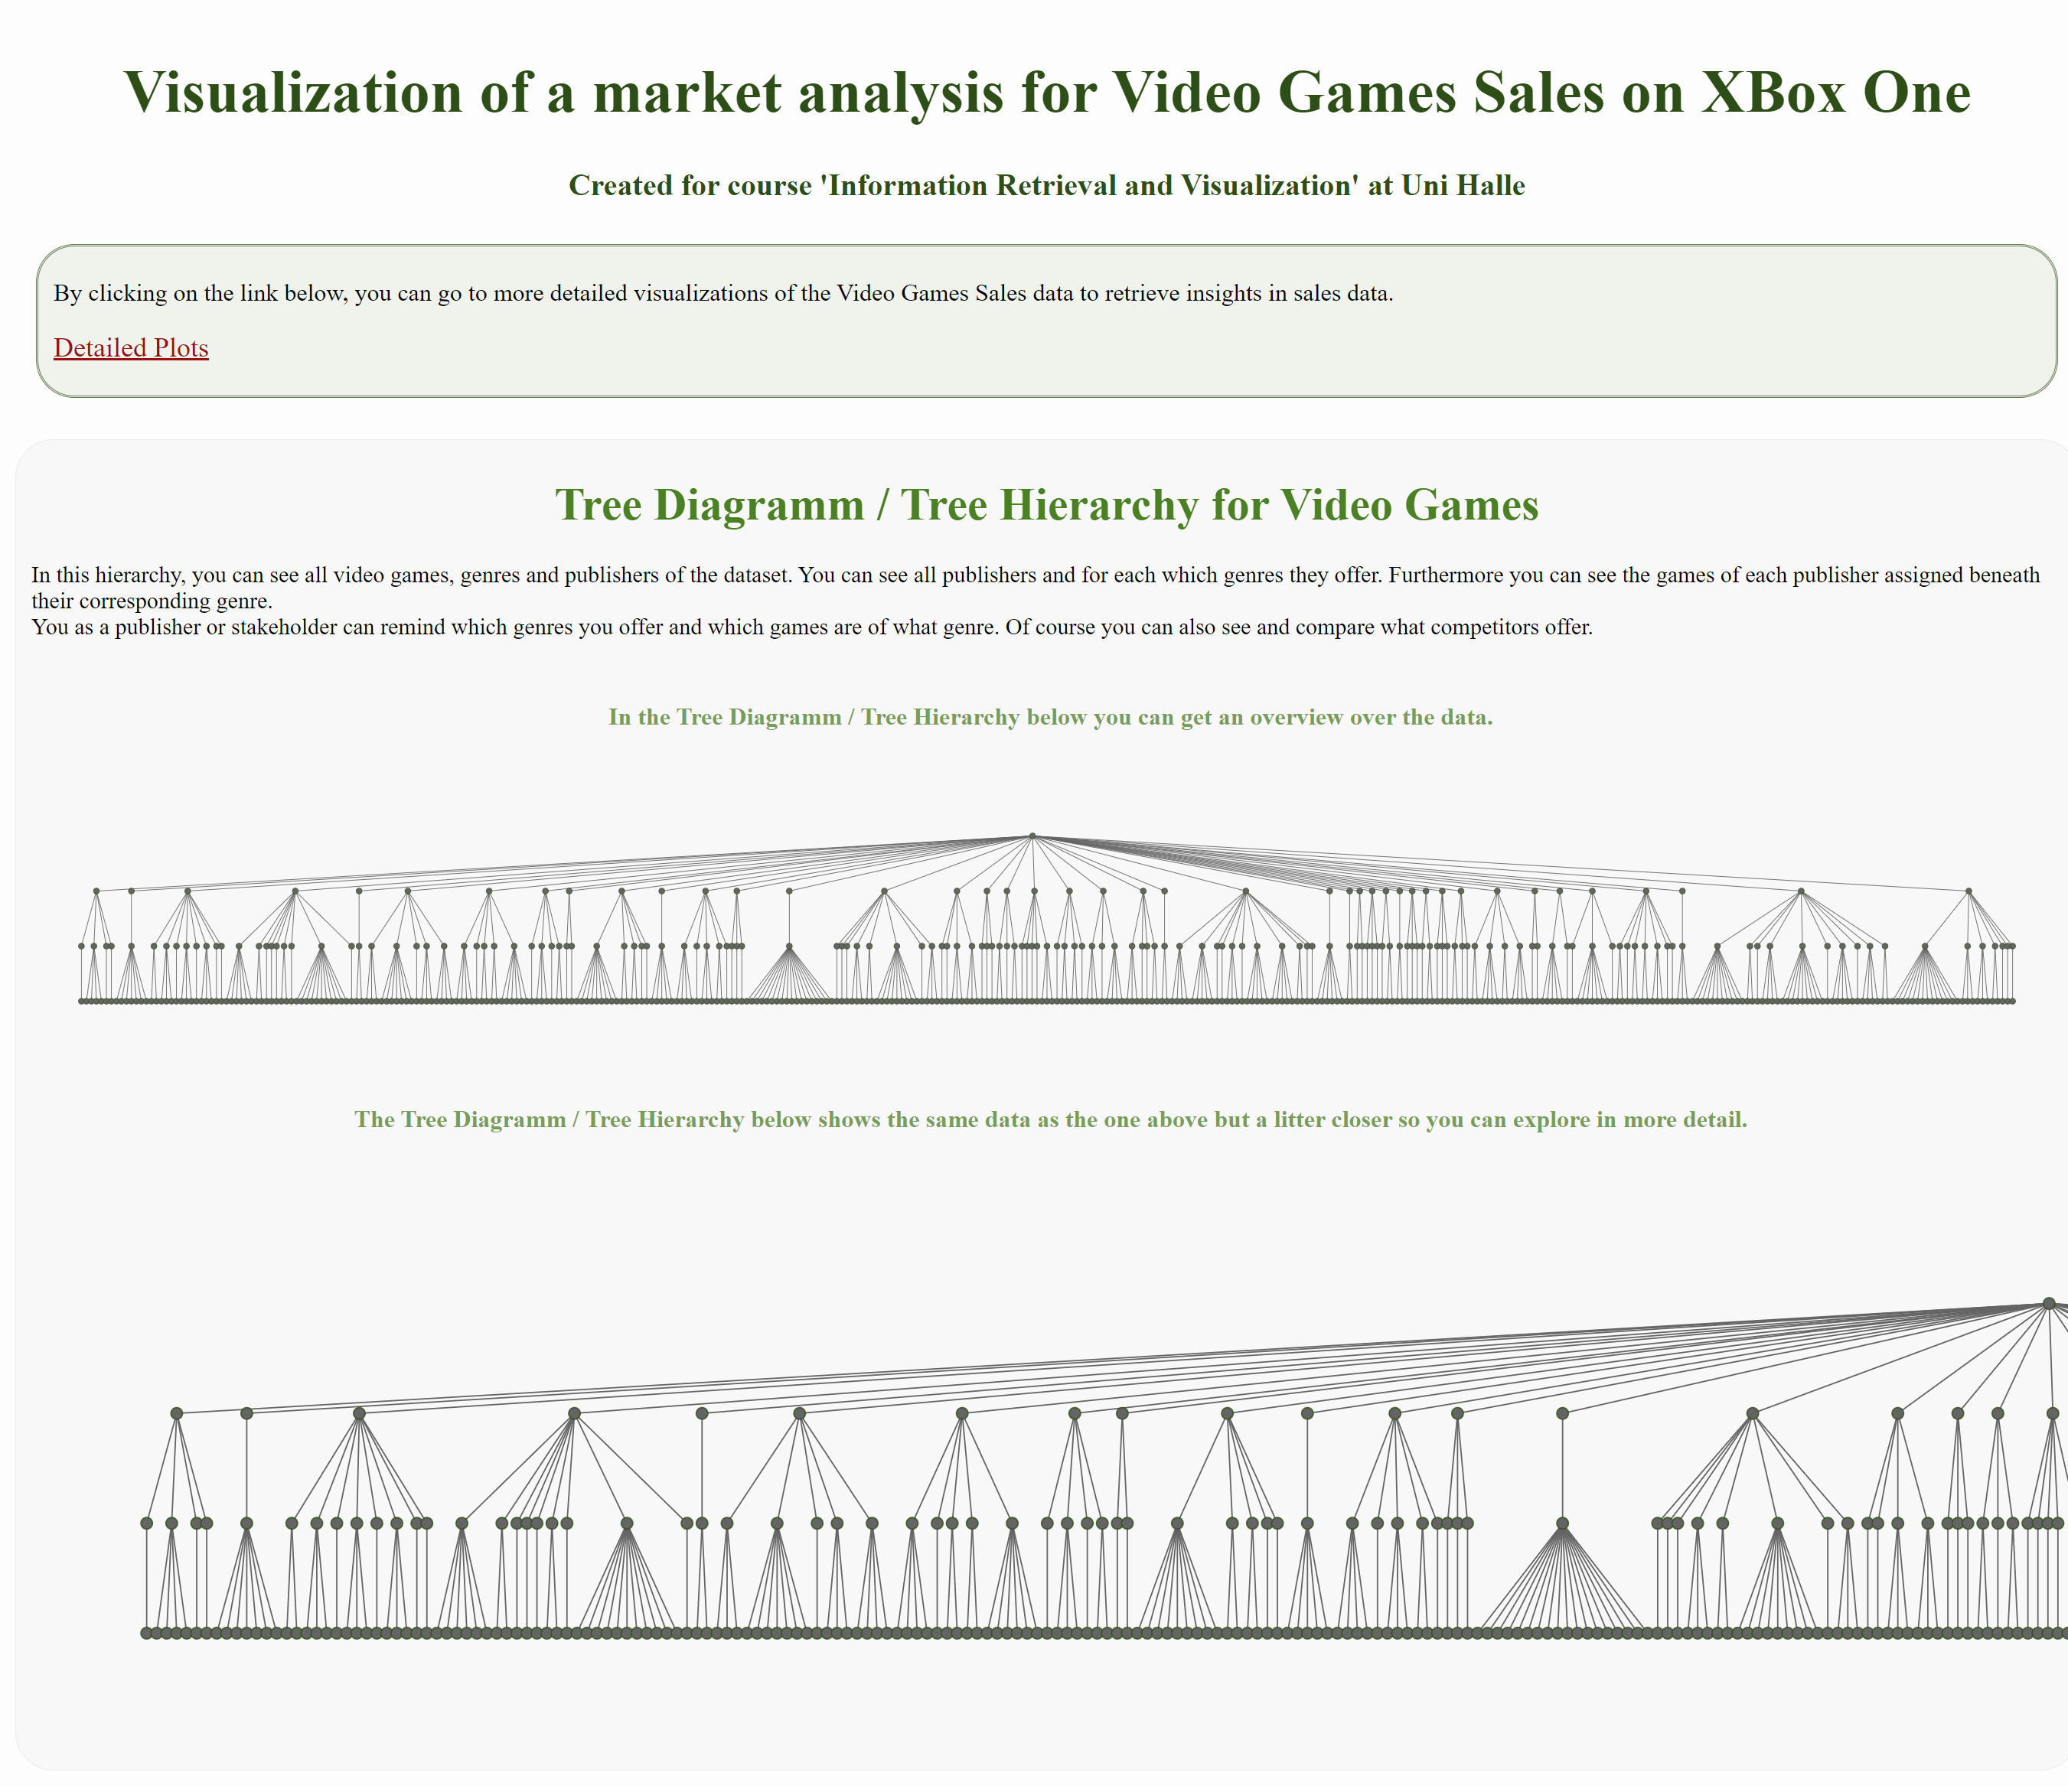
\includegraphics[height=9.5cm]{Bilder/TreeHierarchy_full.png}
        \caption{Gesamte Anzeige des expliziten Baumdiagramms}
        \label{fig:TreeHierarchy}
\end{figure}
Um ungewollten Kreuzungen der Pfade zwischen Publishern und Genres zu verhindern, wird letzteren zur eindeutigen Identifikation das Kürzel des zugehörigen Publishers hinzugefügt.
Andernfalls verlöre die Visualisierung ihre Übersichtlichkeit und die einfache Betrachtung der eigenen abgedeckten Genres und Titel und der Vergleich mit der Konkurrenz.
Eine erste Eingrenzung der Genres durch oben genannte Analysen ist so möglich.

Die aufgeführten Anforderungen an Expressivität, Effektivität und Angemessenheit werden durch ein explizites Baumdiagramm gut erfüllt.
So ist eine zweifelsfreie Darstellung der Beziehungen und Abbildung der Hierarchien möglich, ohne unpassende Assoziationen zu wecken. 
Alle Informationen, die hier für die obere visuelle Ebene der Informationen nötig sind, werden übermittelt. 
In den Daten versteckte Beziehungen werden offengelegt und konkrete Details durch die Anzeige der Knotenbezeichnungen beim Hovern mit der Maus aufgeführt.
Durch das intuitive, schnelle Verständnis ohne notwendige Erklärungen und Legenden, die überblicksartige Ansicht und die weite Verbreitung solcher Diagramme in vielen unterschiedlichen Bereichen ist auch die Effektivität der Visualisierung hinreichend gegeben. 
Die durch Hovern angezeigten expliziten Informationen sowie die schnelle quantitative Übersicht über Angebote durch Zählung der von einem Elternknoten ausgehenden Pfade trägt unter anderem dazu bei.
Weiterhin ist diese Visualisierungstechnik durch den eher als gering einzuschätzenden monetären und zeitlichen Aufwand zur Erstellung bei starker Expressivität und Effektivität angemessen.

Wie erwähnt, wird durch das explizite Baumdiagramm die Anforderung an die Darstellung von hierarchischen Beziehungen erfüllt.
Durch den Einsatz des Walker-Algorithmus wird die Effektivität dank einheitlicher Positionierung der Knoten nochmals verbessert.\cite[688ff.]{Walker.1990}
Vermindert wird sie gleichzeitig durch die hohe Anzahl an Knoten, die zu einem breiteren, leicht weniger übersichtlichem Diagramm führen. 
Durch das Duplizieren des Diagramms mit veränderter Größe wird der Nachteil der größeren Menge an Knoten reduziert.

Hyperbolische Bäume sind eine Alternative zum expliziten Baumdiagramm. 
Durch die Zeichnung der Beziehungen und Knoten im hyperbolischen Raum und einen wachsenden Kreisumfang bietet diese Technik mehr Platz für größere Hierarchien.\cite[2f.]{Lamping.1995}
Jedoch zöge diese Alternative einen höheren (Kosten-) Aufwand mit sich, weniger Intuitivität in der Erkennung der eigenen und konkurrierenden Angebote sowie eine suboptimale quantitative Übersicht der qualitativen Daten. 
Implizite Baumdiagramme sind eine weitere Alternative, bei der die Eltern-Kind-Beziehung durch Umschließung des Kindknotens durch den Elternknoten visualisiert werde.\cite[394]{Schulz.2011}
Sie sind platzsparender, aber durch einen geringeren Bekanntheitsgrad in der Zielgruppe weniger intuitiv verstehbar. 
Als Überblick bieten sie zudem weniger schnell eine Übersicht über eigene und konkurrierende Angebote statt eines Entlangfahrens der Kanten mit dem Auge.

\subsubsection{Visualisierung Zwei}
Für die erste Teilbearbeitung der zweiten Anwendungsaufgabe wird der Parallele Koordinaten Plot gewählt, da er sich gut für Visualisierungen von Datenverteilungen und Abhängigkeiten zwischen Attributen eigne.\cite[11]{Chan.2006}
In positiver Richtung der y-Achse werden parallel zueinander die in ihrem Wertebereich linear skalierten Achsen positioniert.
Ein Datenpunkt hat verschiedene Koordinaten, mittels derer Polygonzüge konstruiert werden.
Die Schnittpunkte mit den jeweiligen Achsen zeigen den Attributwert.\cite[25f.]{Inselberg.1987}~\cite[11]{Chan.2006}

Auf den parallelen Achsen werden die Wertebereiche der Verkaufszahlen der fünf verschiedenen Regionen skaliert und nebeneinander angeordnet abgebildet.
Die Schnittpunkte der Polygonzüge, resp. Datenpunkte, mit den Achsen kodieren die jeweiligen Attributausprägungen in den Regionen.
Mehrdimensionalität und ein ganzheitlicher Blick werden erfüllt.

Es können sowohl die expliziten Details zu Videospielen und ihren Verkaufszahlen als auch die in den Daten versteckten Informationen zu Muster- und Clusterbildung, Abhängigkeiten zwischen mehreren Regionen und Ausreißer offengelegt werden.
Ersteres wird durch die Anzeige der Informationen bei Hovern über ein Polygonzug über dem Plot visualisiert. 
Zweiteres durch die Verbindung der Attributausprägungen eines Titels durch Polygonzüge sowie die sich durch Überschneidungen, Überlappungen und Ansammlungen der Linien bildenden Muster (s. Abb. 2). 
\begin{figure}[h]
        \centering
        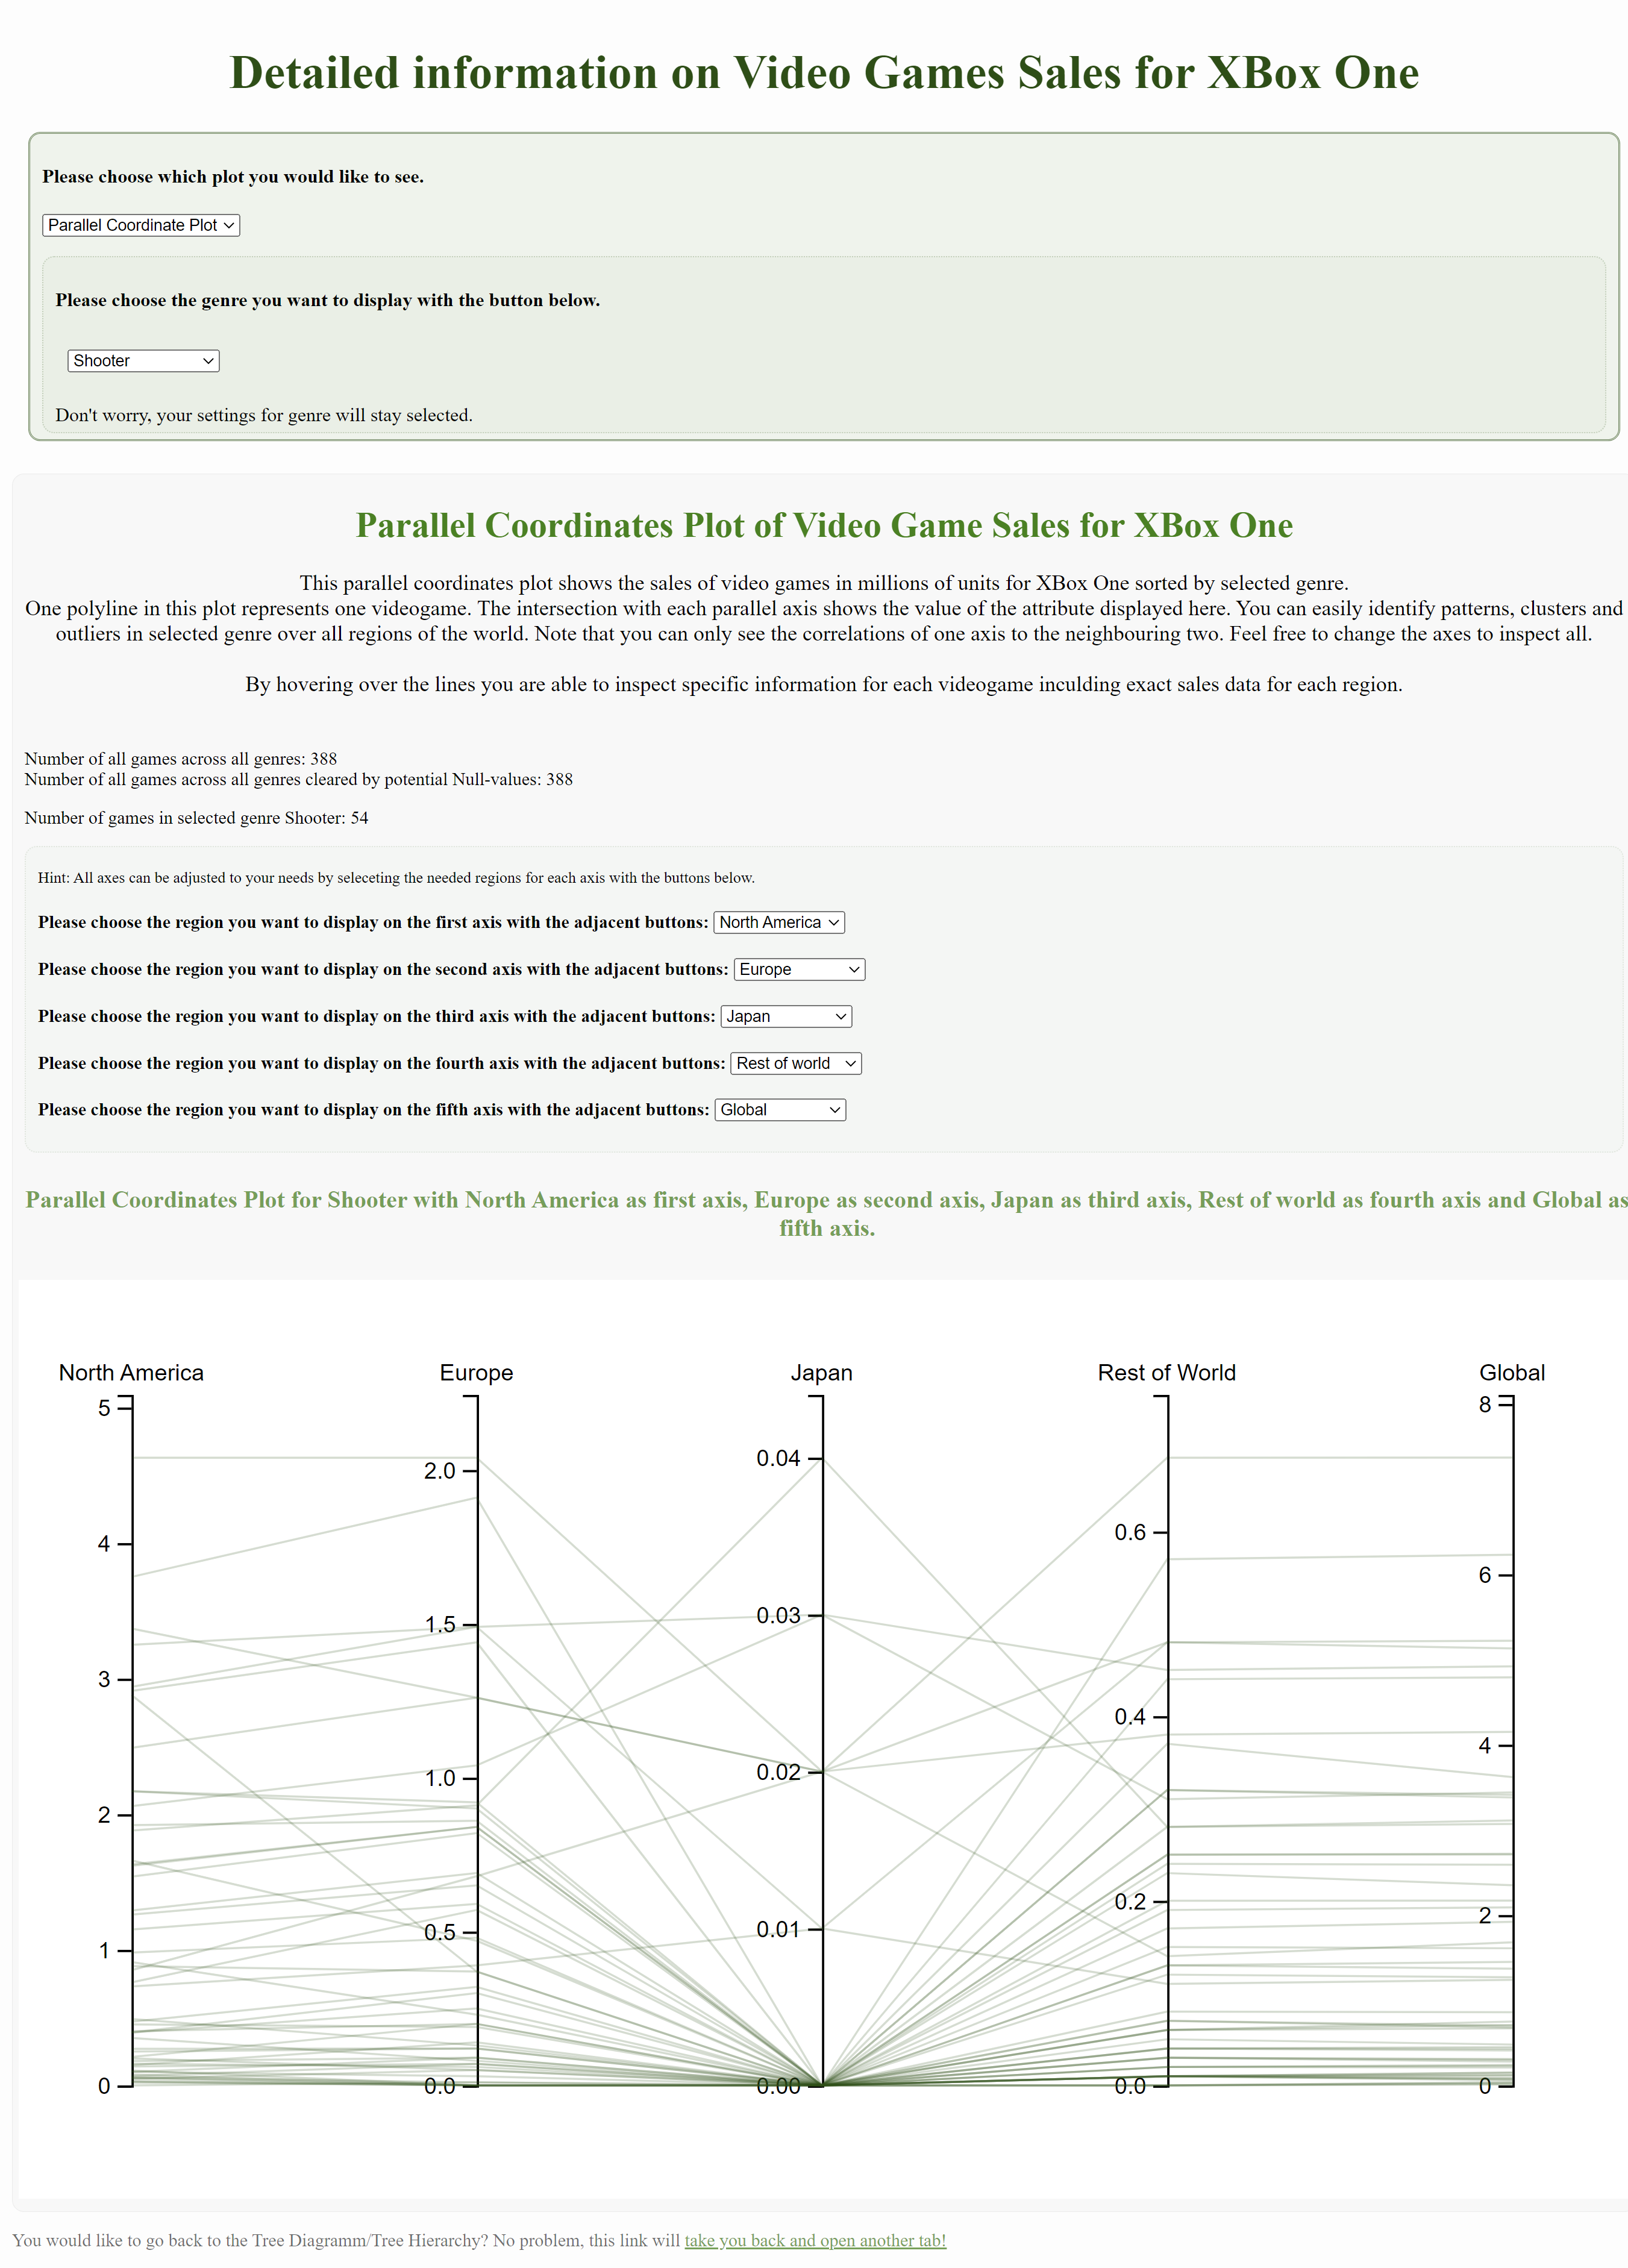
\includegraphics[height=10cm]{Bilder/ParallelPlot_full.png}
        \caption{Gesamte Anzeige des Parallelen Koordinaten Plots}
        \label{fig:ParallelPlot}
\end{figure}
Weiterhin eignet sich die Technik durch die Abbildung der Attributwerte auf Position und in gewissem Maße Orientierung gut für quantitative Daten.\cite{Bertin.1982}
Durch eine freie Wahl der Achsenbelegungen mittels Drop-Down-Menü aller Achsen können zudem weitere interessante Muster, um den gesamten erwünschten Blick von oben zu erhalten, erkannt werden. 
Das Problem der laut Lehman bestehenden Darstellung von Abhängigkeiten nur zwischen drei benachbarten Achsen kann somit umgangen werden.\cite[594]{Lehmann.2010}
Die Expressivität wird insgesamt gut erfüllt.

Muster, Cluster und Ausreißer lassen sich grundlegend gut durch die Polygonzüge erkennen. 
Nichtsdestotrotz wird die Effektivität leicht gemindert, da das korrekte Verständnis der Kodierung der Daten einigen Personen der Zielgruppe schwieriger fallen kann.
Umso wichtiger ist die zuvor beschriebene Möglichkeit zur Wahl der Achsenbelegung sowie prägnanter Erklärtexte.
Bei großen Datensätzen ist es in Parallelen Koordinaten Plots problematisch, einzelne Polygonzüge durch Überlagerungen zu verfolgen.
Durch ein Hervorheben der Linie und der Informationsanzeige beim Hovern kann dies gelöst werden. 
Gleichzeitig erhalten alle Polygonzüge eine grüne Färbung mit geringerer Opazität, sodass Schnittstellen und Häufungen von Liniensegmenten durch einen kräftigeren Ton leicht erkennbar sind. 
Diese Art von Röntgenstrahlentechnik kann die Erkennung von Mustern und Clustern verbessern und verbessert die Effektivität wieder.
Das Design der Visualisierung mittels Filterung und freier Wahl der Achsenbelegung verhindert zwar nicht die vielen Kombinationsmöglichkeiten, jedoch die dabei mittels einfachen Achsentausches auftretende Überforderung.
Parallele Koordinaten Plots sind zwar etwas (kosten-) aufwendiger zu erstellen, bleiben aber trotzdem im Kontext der Anwendungsaufgabe angemessen.

Eine Alternativen zu Parallelen Koordinaten Plots stellen Icon-Techniken, bspw. Star Plots oder Stickfigures dar.
In Star Plots seien die Dimensionen als eckige Achsen ausgehend von einem Kreismittelpunkt mit einer äußeren Verbindungslinie zur Repräsentation der Attributausprägung jeder der Dimensionen visualisiert.
Dabei steigt jedoch die Anzahl der zu erstellenden Icons mit steigernder Menge an Datenpunkten stark, da sie nur je einen Datenpunkt repräsentieren können.\cite[20]{Chan.2006}
Ein ähnliches Problem existiert auch bei Stickfigures, die zusätzlich durch zwei Attribute in einem Koordinatensystem mit weiteren positioniert werden.
Zwar können so grobe Muster und Cluster erkannt werden, die anderen Anforderungen bspw. konkrete Informationen zu Datenpunkten werden allerdings unzureichend erfüllt.
Intuitivität und Effektivität sind im vorherrschenden Kontext unzureichend, womit Icon-Techniken alternativ ungeeignet sind. 

\subsubsection{Visualisierung Drei}
Die vollständige Beantwortung der zweiten Anwendungsaufgabe bedingt eine weitere Visualisierung, für die die Technik des Scatterplots gewählt wird.
In einem kartesischen Koordinatensystem mit orthogonaler x- und y-Achse werden x- und y-Werte 
zweier variabler Attribute eines Datenpunkts zu bivariaten Paaren zusammengefasst.
Durch die Positionierung dieser als Punkte im Koordinatensystem werden die Attributwerte visualisiert.\cite[103]{Friendly.2005}
Mittels Abtragung vieler Datenpunkte werden Form der Abhängigkeiten, Muster und Ausreißer zwischen zwei Attributen sichtbar.\cite[9]{Chan.2006}~\cite[103]{Friendly.2005}
Die Schwäche des Scatterplots durch Verlust an Informationen von mehreren Dimensionen wandelt sich in diesem Fall durch eine Detaillierung und Überprüfung der Erkenntnisse des Parallelen Koordinaten Plots zum Vorteil.\cite[9]{Chan.2006}~\cite[93]{Wegman.1997}

Im diesem Scatterplot ist die Belegung der Achsen zur Darstellung der Wertebereiche der Attribute \textit{North America}, \textit{Europe}, \textit{Japan}, \textit{Rest of World} und \textit{Global} frei wählbar, 
um den Anforderungen nach Auswahl interessanter Attribute des Parallelen Koordinaten Plots zur Detaillierung dieses nachzukommen (s. Abb. 3).
\begin{figure}[h]
        \centering
        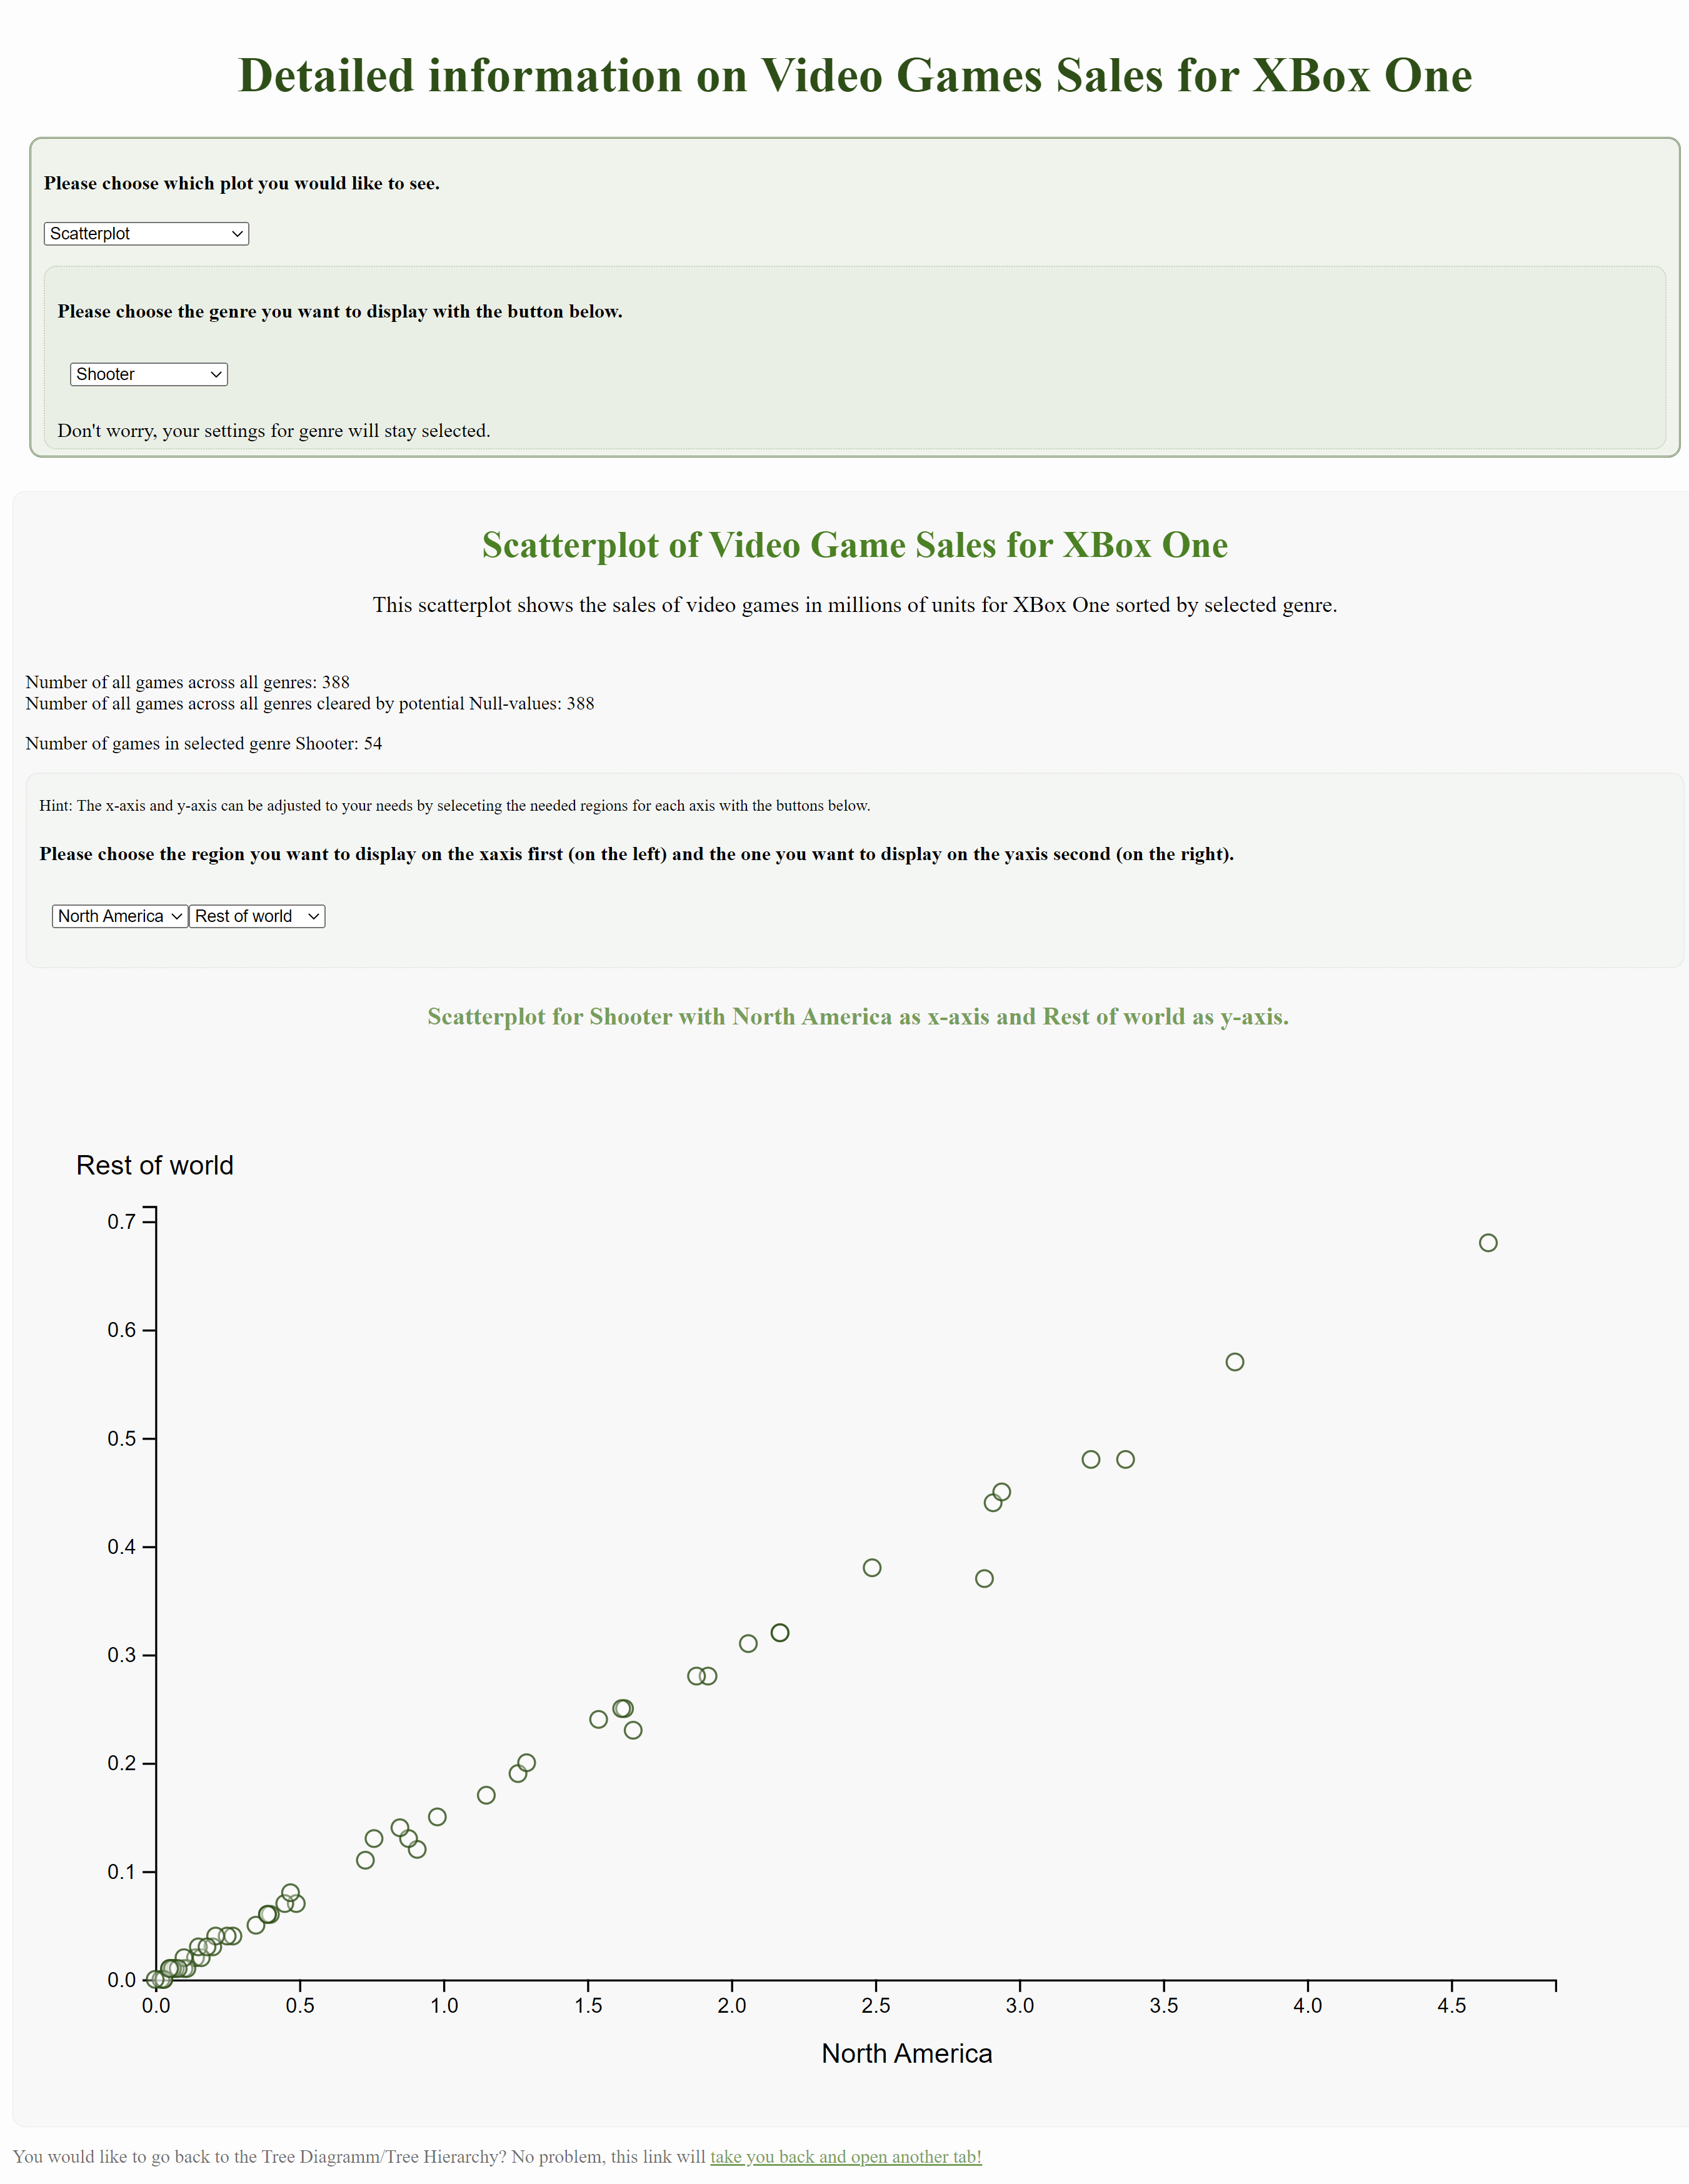
\includegraphics[height=8.5cm]{Bilder/Scatterplot_full.png}
        \caption{Ausschnitt des Scatterplots}
        \label{fig:Scatterplot}
\end{figure}
Zudem sind Abhängigkeiten zwischen allen Attributkombinationen untersuchbar. 
Die Datenpunkte werden zur visuellen Ablesbarkeit wie oben beschrieben als Attributwert-Kombinationen kodiert, 
an den Achsen skaliert und als klassische Kreise im Raum des Koordinatensystems positioniert. 
Quantitative Daten lassen sich am besten auf Position und untergeordnet auch auf Orientierung abbilden, 
was der Scatterplot bestens umsetzt.\cite{Bertin.1982}

Die Anforderungen an die Expressivität auch bezüglich der oberen visuellen Ebene der Informationen werden durch die 
unmissverständliche Zuweisung der Videospielinformationen zum Punkt im Diagramm mittels Hovern sowie die Visualisierung von versteckten Informationen erfüllt. 
Letztere bestehen aus dem Aufzeigen der Art der Korrelationen, Clustern und Ausreißern zwischen zwei wählbaren Attributen.
Weiterhin lässt sich mit ihm die gewünschte Vergrößerung der multidimensionalen Daten auf eine Ansicht von nur zwei Attributen und der damit verbundene höhere Detaillierungsgrad umsetzen. 
Die Analyse des komplizierteren Parallelen Koordianten Plots kann überprüft und Fehler erkannt werden. 
Detailfragen zur finalen Entscheidung für ein weiter zu fokussierendes Genre oder eventuelle Korrelationen zwischen Regionen in diesem, 
die hinder- oder förderlich sein können, werden beantwortet. 
Durch eine deutliche räumliche Abgrenzung von Punkthaufen jeder Form können Cluster erkannt, bestätigt und einzelne Ausreißer bestimmt werden.
Diese konkreten Anforderungen werden damit erfüllt.

Effektivität und Angemessenheit sind klar gegeben. 
Ersteres ergibt sich aus der starken Verbreitung der Technik in allen Bereichen und der unmissverständlichen, sich durch die Positionierung der Punkte ergebenden Darstellung. 
Damit visualisiert der Scatterplot intuitiv und schnell lesbar eine Fülle an detaillierten statistischen Informationen.
Er ist durch seine Trivialität in der Abbildung zweier quantitativer Attribute angemessen. 
Bei hoher Expressivität und Effektivität ist der Scatterplot vergleichsweise unkompliziert und kostengünstig.

In diesem Kontext sind keine sinnvollen Alternativen möglich. 
Korrelationstabellen listen Abhängigkeiten nur tabellarisch auf, visualisieren sie jedoch nicht mittels einer spezifischen Technik.
In QQ-Plots können zwei statistische Variablen miteinander verglichen werden, allerdings durch geordnete Gegenüberstellung ihrer Quantile zur Erkennung von Verteilungen.
Dies dient nicht der Lösung des Zielproblems, könnte aber in einerzu beauftragenden detaillierteren Marktstudie Verwendung finden.
So sei der Scatterplot „the most versatile, polymorphic, and generally useful”\cite[103]{Friendly.2005} Visualisierung für statistische Daten und 
eignet sich perfekt zur abschließenden Beantwortung der zweiten Anwendungsaufgabe und des gesamten Zielproblems.

\subsection{Interaktion}
In jeder Visualisierung sind Interaktionen mittels Hovern über die Datenpunkte zur Anzeige konkreter Informationen im jeweiligen Kontext des Plots 
sowie zum Aufleuchten des Datenpunkts zur besseren Erkennung möglich.
So werden die Anforderungen an stets mögliche Detailansichten sowie Verbesserungen von Expressivität und Effektivität wie zuvor beschrieben erfüllt. 

In jeder einzelnen Visualisierung sind weitere Interaktionsmöglichkeiten integriert. 
So kann im expliziten Baumdiagramm der vergrößerte Baum mittels Scrollbar verschoben und mithilfe eines Links zu den detaillierteren Visualisierungen gewechselt werden.
Von jeder der detaillierten Plots kann der Anwender durch einen Link am unteren Ende der Website schnell einen weiteren Tab zur Rückkehr zum Baumdiagramm als Ausgangspunkt und Übersicht für bspw. einen Abgleich öffnen.
Im Parallelen Koordinaten Plot sind die Achsen dank eines Drop-Down-Menüs für jede frei belegbar. 
Wie in Kapitel 3.3.2 beschrieben, kann dies Überforderung, Unübersichtlichkeit und Zeitverlust durch bloßen Achsentausch verhindern 
sowie die teils versteckten Abhängigkeiten zwischen den Regionen in jeder Kombination sichtbar machen. 
Die Betrachtung der Abhängigkeiten zwischen nur drei benachbarten Dimensionen ist so weniger problematisch.
Auch der Scatterplot bietet die Interaktion mit je einem Button als Drop-Down-Menü zur freien Achsenbelegung, 
um detaillierte Untersuchungen von Abhängigkeiten und Vergleiche zwischen zwei beliebigen Attributen zu ermöglichen.
Dies dient zudem der gewünschten Vergrößerung und Detaillierung der vorherigen Visualisierung.

Ist der Anwender bei den detaillierten Plots angelangt, kann er mit einem Button als Drop-Down-Menü interagieren 
und mit diesem leicht und schnell zwischen allen Visualisierungen wechseln.
Bei einem Wechsel zum Baumdiagramm leitet der dort platzierte Link zur eigentlichen Visualisierung dieses weiter. 
Für eine verbesserte Effektivität, Zeitersparnis und Komfort bleiben die Achsenbelegungen bei einem Plotwechsel mittels Drop-Down-Menü gespeichert 
und müssen bei erneutem Wechsel zurück nicht neu eingestellt werden. 
Welche Attribute auf den Achsen ausgewählt sind, ist durch eine sich anpassende Unterüberschrift des Plots gekennzeichnet. 

Zuletzt wird die Anforderung an einen Filter zur Auswahl der Genres und entsprechender Eingrenzung der Stichprobe in den Visualisierungen Paralleler Koordinaten Plot und Scatterplot umgesetzt (s. Abb. 4).
Hierzu gibt es bei beiden Visualisierungen die Möglichkeit zur Interaktion mit einem Drop-Down-Menü, 
in dem das gewünschte zu betrachtende Genre unter Anpassung der visualisierten Daten ausgewählt werden kann.
Die Filterung bleibt bei Umschalten des Plots bestehen und wird direkt auf den anderen angewandt, 
sodass eine Interaktion mit einem Plot zur Änderung des anderen führt. 
Durch die Anzeige des Menüs sowie die sich anpassende Unterüberschrift des Plots ist das gewählte Genre nachvollziehbar.
\begin{wrapfigure}{r}{5cm}
        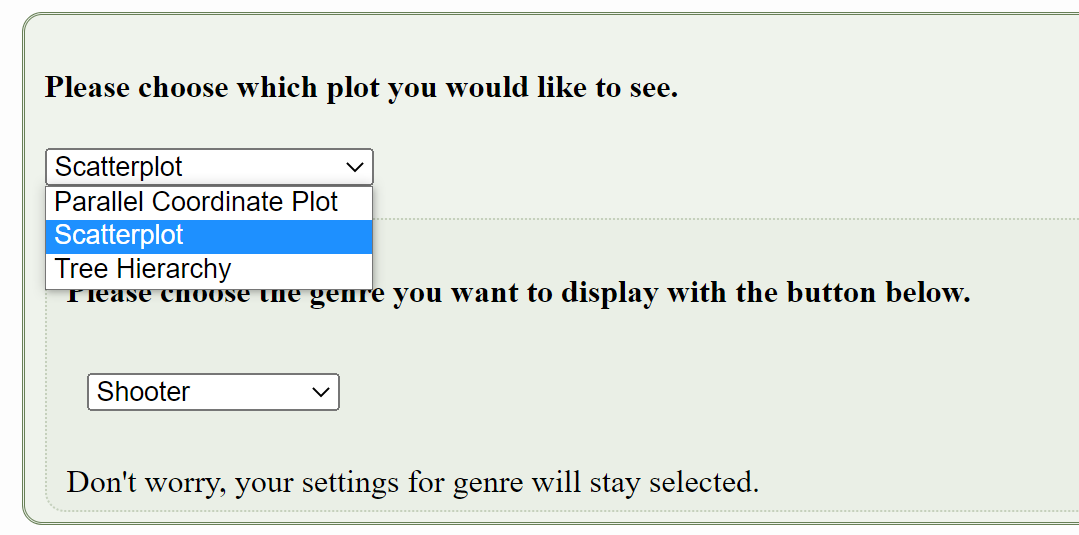
\includegraphics[width=4.5cm]{Bilder/filters_global.png}
        \caption{Filter}
        \label{fig:Filter}
\end{wrapfigure}
Die Zielgruppe kann durch die Interaktion mittels Genrefilter die Spiele und die Abhängigkeiten derer zwischen den Regionen sinnvoller vergleichen 
und vielversprechende Genres und in diesen möglicherweise Regionen für die Investition in weitere Marktstudien eingrenzen.

\section{Implementierung}
Nachfolgend wird die Implementierung der präsentierten Visualisierungen und Interaktionen beschrieben. 
Der Code unterteilt sich in fünf Elm-Module, in denen die drei einzelnen Visualisierungen, die Datenstrukturen 
und die Zusammensetzung und Ausführung des Hauptprogramms implementiert sind. 
\textit{TreeHierarchy} dient als Ausgangspunkt, wobei \textit{MainScatterParallel} den Hauptteil der Anwendung durch die eigentliche Verbindung 
der Visualisierungen enthält.
Es werden verschiedene Bibliotheken genutzt, die je zu Beginn des Moduls importiert werden.
           
Die Implementierung zeigte sich als zeitaufwendig, da trotz umfangreicher Übungsaufgaben die Routine im Programmieren mit Elm fehlte.
Die Übungsaufgaben waren jedoch hilfreich und dienten oft als Grundlage der Funktionen.
Im gesamten Projekt gab es neue Erkenntnisse und Verständnis für die Funktionen der Sprache und des Übungsquellcodes, 
sodass sich ein großer zusätzlicher Lerneffekt einstellte.
Trotz der guten Abgabevorlagen der Autorin zu den Übungsserien traten Schwierigkeiten auf, 
die in den folgenden Unterkapiteln Erwähnung finden.
          
\subsection{Data.elm}
\textit{Data} dient der Deklaration fast aller verwendeten Datentypen sowie der Decodierungen. 
Nur \textit{Model} und \textit{Msg} sind aus Verständnisgründen des Quellcodes in \textit{MainScatterParallel} definiert. 

Zunächst wird mit \textit{decodeGameSales}, \textit{csvString\_to\_data} und \textit{gamesSalesList} die Decodierung der Felder der CSV-Dateien 
als String bzw. Float implementiert und in eine Liste vom Typ GameSales geschrieben. 
Darauf folgt die Decodierung der JSON-Datei mittels \textit{treeDecoder}.
Beide Decoder finden im \textit{update} in \textit{MainScatterParallel} zur initialen Überschreibung der Daten ihre Anwendung.
Sie basieren auf den für die Übungen sieben und neun verwendeten Decodern und wurden an die hier verwendeten Daten angepasst.

Es folgt die Deklaration der für alle Visualisierungen außer \textit{TreeHierarchy} wichtigen Datentypen.
\textit{Type alias GameSales} definiert die grundlegenden Datentypen der CSV-Datei, die u. a. im Model in \textit{MainScatterParallel} weiterverwendet werden. 
Der \textit{type RegionType} und der \textit{type PlotType} als CustomTypes dienen der Achsenauswahl in den Visualisierungen zwei und drei 
sowie der Wahl der anzuzeigenden Visualisierung. 
Es folgen die durch die Übungen bekannten Datentypen für die spezifischen Visualisierungen. 
Zuletzt werden die für die Buttons wichtigen Funktionen zur Konvertierung eines Strings zum jeweiligen CustomType 
und mit Ausnahme vom PlotType umgekehrt beschrieben. 
Dies dient der Erstellung von nur Strings erlaubenden Buttons und der bspw. resultierenden korrekten Anzeige von aktuell ausgewählten Regionen.
Die Konvertierung eines RegionType zu einem Tupel aus GameSales und Float für \textit{multiDimenData} in \textit{ParallelPlot} nötig.

\subsection{TreeHierarchy.elm}
Für das Modul können große Teile des von der Autorin in Übungsserie neun erstellten Quellcodes unter minimaler Anpassung an die verwendeten Daten genutzt werden.
Nach der Definition der \textit{main}-Funktion wird die Anwendung initialisiert, 
die Daten unter Anwendung des JSON-Decoders geladen und die jeweils auszuführenden Aktionen bei korrektem oder inkorrektem Laden der Daten bestimmt. 
Es folgt die Helferfunktion \textit{convert} zur Konvertierung des Baumes basierend auf den Vorgaben zu Übung neun.

\textit{TreePlot2} zur Zeichnung des Baumes ohne Scrollen und \textit{treePlot} zur näheren Ansicht des Baumes werden folgend implementiert. 
Sie unterscheiden sich einzig in der prozentualen Vergrößerung der global definierten Höhen und Breiten um 200 bzw. 150 Prozent im \textit{treePlot}.
Mittels lokaler Funktionen wird das Layout des Baumes bestimmt, bevor die Abhängigkeiten mit Hilfe von \textit{Dict.get} 
zum Erhalt der x- und y-Werte berechnet werden, um die Pfade zwischen Eltern- und Kindknoten zu zeichnen. 
Die Funktionen \textit{checkRootNegative} und \textit{nodeValuesPath} verhindern das fehlerhafte Zeichnen einer Linie zum nicht existenten Elternknoten der Wurzel.
Nachfolgend werden die berechneten Verbindungen durch Anwendung zuvor global implementierter Funktion \textit{line} auf \textit{nodeValuesPath} gezeichnet.
Berechnete Knoten werden durch Anwendung von zuvor definiertem \textit{point} auf \textit{nodeValues} mit einer fett gedruckten, um 75° rotierten Beschriftung visualisiert. 
Das Design wird im global definierten CSS \textit{cssTree} vorgenommen. 

In der \textit{view}-Funktion werden die Daten in einen Baum konvertiert, 
bevor dieser mit dem CSS den beiden Plotfunktionen des Baumes übergeben wird.
Anordnung sowie der Design der HTML-Elemente sind an \textit{MainScatterParallel} angepasst. 
Zuletzt werden allgemeine, konstante Einstellungen zum Plot definiert, die abgesehen von bestimmten Werten
auf den Vorgaben der Vorlage zum Arbeiten mit Bäumen und den Abgaben der Autorin zu Übung neun basieren.

Die Implementierung der expliziten Baumdarstellung bereitete keine Schwierigkeiten, 
da sehr viel auf den abgegebenen Quellcodes der Autorin zu Übung neun basiert. 
Lediglich der Decoder musste an die Datenfelder angepasst, der Link zum Laden der Daten geändert, das CSS global definiert 
sowie die besten Design- und Darstellungsweisen mit zweifacher Darstellung des Baumes gefunden werden. 
Das Seitendesign im \textit{view} wurde an jenes des \textit{MainScatterParallel} angepasst. 

\subsection{ParallelPlot.elm}
Der \textit{ParallelPlot} enthält zunächst drei Funktionen zur Zuordnung der Daten zum benötigten Datentyp und der Reduzierung der Datensätze um solche, 
die Null-Values enthalten. 
Letzteres ist durch die manuelle Datenvorverarbeitung zwar nicht zwingend notwendig, 
schließt jedoch Fehler aus und es kann auf Änderungen der Rohdaten eingegangen werden. 

Die erste Hilfsfunktion dient mittels \textit{Maybe.map2} dem Pipen.
Basierend auf einer normalen \textit{Maybe.map5} Funktion wird die zweite Hilfsfunktion um einen Parameter erweitert. 
Beide begründen sich aus den Elm-Core-Bibliothek-Dokumentationen zu Maybe.\cite{EvanCzaplicki.o.J.} 
Aufgrund des fehlenden \textit{Maybe.map6}, wird zum Umgehen des Problems in \textit{helpMapBig} die erste Hilfsfunktion angewandt. 
\textit{AssignmentAndReduce} wandelt schließlich lokal mittels \textit{helpMapBig} die Daten vom Typ GameSales zu Maybe GameSales 
und reduziert sie um die Datensätze mit fehlenden Werten mittels \textit{List.filterMap}.
Diese Funktion basiert auf den Abgaben der Autorin zu Übung sechs.

D\textit{MultiDimenData} dient zusammen mit der lokalen Funktion \textit{multiDimFunction} aus \textit{MainScatterParallel} 
der freien Achsenbelegung.
Das Grundgerüst beider Funktionen basiert auf den Abgaben der Autorin zu Übung sechs, 
wobei der dortige Achsentausch für die Anforderungen an die Visualisierungen geändert wurde. 
\textit{MultiDimenData} benötigt eine Liste von GameSales, fünf RegionTypes als auszuwählende Regionen für die Achsen, 
den Namen des Spieles und seinen Publisher als String zur Anzeige dieser im späteren Plot. 
Zusätzlich sind fünf Namen, also Beschriftungen als String nötig. 
Die Begründung liegt in der Definition der Recordfelder in \textit{type Model} sowie den für das \textit{update} benötigten Datentypen 
\textit{(RegionType, String)}.
Die Funktion gibt den Typ \textit{MultiDimData} zur Übergabe an \textit{scatterplotParallel} aus. 
Eine besondere Schwierigkeit in der Konstruktion lag im Umfang und Verständnis der nötigen Datentypen. 
So muss der RegionType innerhalb der Funktion mittels \textit{regionTypeToAxisAnnotation} umgeschrieben werden, 
um zu \textit{MultiDimPoint} zu passen und alles schlussendlich als \textit{MultiDimData} auszugeben. 
Die lokale Funktion \textit{multiDimFunction} aus \textit{MainScatterParallel} wendet \textit{multiDimenData} 
letztlich mit den benötigten Daten für die Parameter an.

Der \textit{scatterplotParallel} kann nahezu unverändert aus den Abgaben der Autorin zu Übung sechs übernommen werden. 
Hier werden unter anderem die Achsen parallel zueinander positioniert sowie inklusive Beschriftungen in einem umgebenden Rechteck gezeichnet.
Die Zeichnung der Datenpunkte wird durch \textit{Shape.line} und \textit{Shape.linaerCurve} realisiert.
Der beim Hovern über einen Polygonzug anzuzeigende Text wird in einer lokalen Funktion beschrieben, bevor dieser die entsprechenden Daten übergeben werden.
Im anschließend global definierten \textit{cssParallel} wird die Farbopazität der Datenpunkte zur Erzielung des Röntgeneffektes auf 0.5 festgelegt 
und die stärkere grüne Färbung beim Hovern hinzugefügt. 
Die abschließenden generellen Ploteinstellungen basieren abgesehen von einigen Werten auf den Abgaben der Autorin zu Übung sechs. 
 
Das Zeichnen des \textit{ParallelPlots} bereitete wenig Schwierigkeiten, da sich die Erstellung in weiten Bereichen auf den Abgaben zu Übung sechs stützte.
Komplizierter war zunächst die Implementierung des Mappings und der Filterung nach Null-Werten durch das fehlende \textit{List.map6} 
sowie die Umsetzung der freien Achsenauswahl wie zuvor beschrieben. 
Dabei benötigte es viel Ausprobieren und Verständnis, welche Datentypen für welche weiteren Funktionen benötigt 
und welche als Eingabe möglich waren.

\subsection{Scatterplot.elm}
Für den \textit{Scatterplot} sind beginnend drei ähnliche Funktionen mit demselben Zweck wie in \textit{ParallelPlot} nötig,
wobei sich erstere zwei gleichen und \textit{FilterAndReduceGames} auf den Abgaben der Autorin zu Übung eins basiert, aber ähnlich funktioniert.
Unterschiedlich ist hier die Zuordnung der Eingabedaten zum Typ Maybe Point.
Die gefilterten Daten werden als Output für das Zeichnen des Plots in XyData geschrieben.
Der \textit{regionFilter} stammt aus der vierten Übungsserie der Autorin und filtert unter Eingabe der Liste GameSales und des RegionTypes 
die Datenpunkte nach der gewählten Region zur Interaktion durch freie Achsenbelegung innerhalb des Plots.

\textit{Point} legt die Positionierung und Beschriftung der Punkte für die Weiterverwendung in \textit{Scatterplot} fest.
Der \textit{scatterplot} zeichnet den Plot, bei dem die lokale Funktion \textit{pointsXY} die Variabilität der Achsen und damit x- und y-Werte der Punkte ermöglicht.
Weiterhin wird im \textit{scatterplot} mittels SVG die Positionierung der x- und y-Achse, ihrer Beschriftungen 
und der Punkte mittels \textit{xScaleLocal}, \textit{yScaleLocal} und \textit{pointsXY} sowie der globalen Funktion \textit{point} vorgenommen. 
Der \textit{scatterplot} basiert auf den Abgaben der Autorin zu Übung 1.4 sowie Übung vier für die lokale Funktion \textit{pointsXY}. 
Der \textit{cssPoint} wird global definiert, bevor allgemeine, konstant für den Plot geltende Einstellungen, 
basierend auf den Übungen eins bis vier, folgen. 

Die Implementierung des \textit{Scatterplots} verlief überwiegend problemlos, jedoch langsam durch stetes Überprüfen der richtigen Datentypen.
Schwieriger war wie zuvor die Umsetzung des Mappings und Filterns nach Null-Werten, wobei die Lösung weitgehend aus dem \textit{ParallelPlot} übernommen werden konnte. 
Weiterhin musste, konträr zu den meisten Übungsserien, auf die variable Definition der Achsen zur freien Achsenbelegung geachtet werden.
Entsprechende Zeit- und Denkinvestitionen überwanden die Probleme.

\subsection{MainScatterParallel.elm}
Aufgrund besserer Erkenntlichkeit des Ursprungs von Funktionen aus zuvor beschriebenen Elm-Modulen in \textit{MainScatterParallel}
werden nur die allgemeinen Module importiert. 
Für \textit{MainScatterParallel} wird die gesamte Elm-Architektur verwendet, da das Modul den \textit{Scatterplot} und den \textit{ParallelPlot} ausführen 
und alle drei Visualisierungen verbinden soll.
Zunächst wird das Programm in der \textit{main}-Funktion definiert sowie die \textit{subcritpions-} und \textit{init}-Funktion implementiert.

In \textit{type Model} werden die drei Varianten Error, Loading und Success zur Anzeige in den entsprechenden Fällen beschrieben, 
wobei die Variante Success gleichzeitig ein Record mit den dort beschriebenen Feldern ist. 
Die initialen Werte werden in dieser Implementierung erst durch die \textit{update}-Funktion dort hinein geschrieben.
Im Feld \textit{data} werden die geladenen und decodierten Daten als Liste von GameSales gespeichert. 
Zur Ermöglichung der Interaktionen bestehen die weiteren Felder für das Genre, die Achsen eins bis fünf, 
die Namen der Achsen eins bis fünf, die x- und y-Achse und den gewünschten Plot. 
Der \textit{type Msg} definiert die Varianten zur Überschreibung des Models mittels \textit{update}. 
Es gibt eine Variante zum erfolgreichen Laden und Initialisieren der Daten, je eine für jeden möglichen Achsenwechsel in den Plots und den Plotwechsel an sich.

In der \textit{update}-Funktion werden zuerst die initialen Attributwerte definiert und nach Anwendung der Decodierung in Success gespeichert. 
Weiterhin werden für alle Interaktionen mit dem Model die \textit{Msg}-Varianten beschrieben, 
um die Überschreibung der Variante durch Klick auf einen Button das Model festzulegen.

Nachfolgend sind die Button-Funktionen zur Überschreibung des Models implementiert.
\begin{wrapfigure}{r}{6cm}
        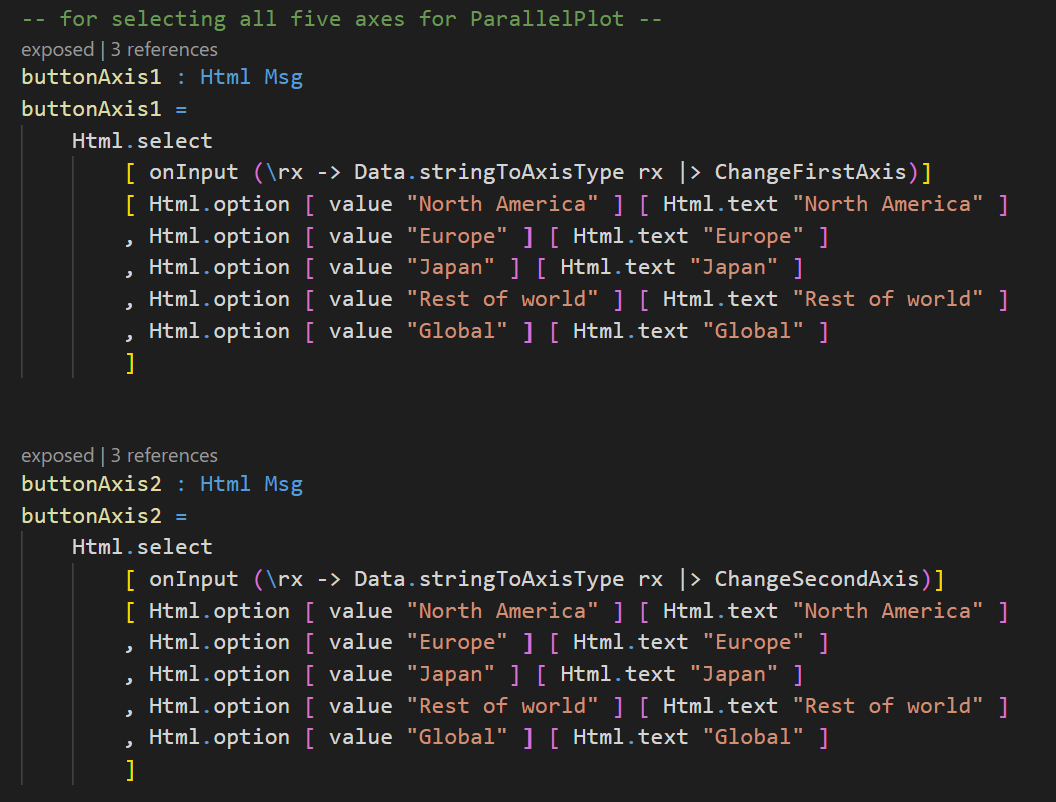
\includegraphics[width=5.5cm]{Bilder/Code_ButtonsForParallel.png}
        \caption{Ausschnitt der Buttons zur Achsenwahl im \textit{ParallelPlot}}
        \label{fig:Buttons}
\end{wrapfigure}
Für alle außer den \textit{buttonGenreType} ist die Nutzung der in \textit{Data} definierten Umwandlungsfunktionen 
von Strings für die Buttons zu den entsprechend definierten Datentypen wichtig. 
Die Änderungen werden in der \textit{Msg}-Variante gespeichert und durch \textit{update} das Model überschrieben.
Die Buttons basieren auf den Abgaben der Autorin aus Übung vier, ebenso die folgende Funktion \textit{filterGenre}. 
Sie wird im \textit{view} zur Filterung nach Genre angewandt.

In der \textit{view}-Funktion werden die Varianten des Models zur Ansicht behandelt, wobei nur auf den Erfolgsfall näher eingegangen wird. 
Zunächst wird eine \textit{let-in}-Konstruktion auf erster äußerer Ebene erstellt. 
In lokalen Funktionen werden \textit{gameSalesData} und die Spieleanzahl insgesamt beschrieben 
sowie der globale \textit{filterGenre} zur Datenfilterung nach Genre angewandt und die Listenlänge berechnet. 
Zum Wechsel zwischen den Plots werden die Varianten des Datentyps \textit{PlotType} im \textit{in}-Teil angelegt (s. Abb. 6). 
\begin{figure}[h]
	\centering
        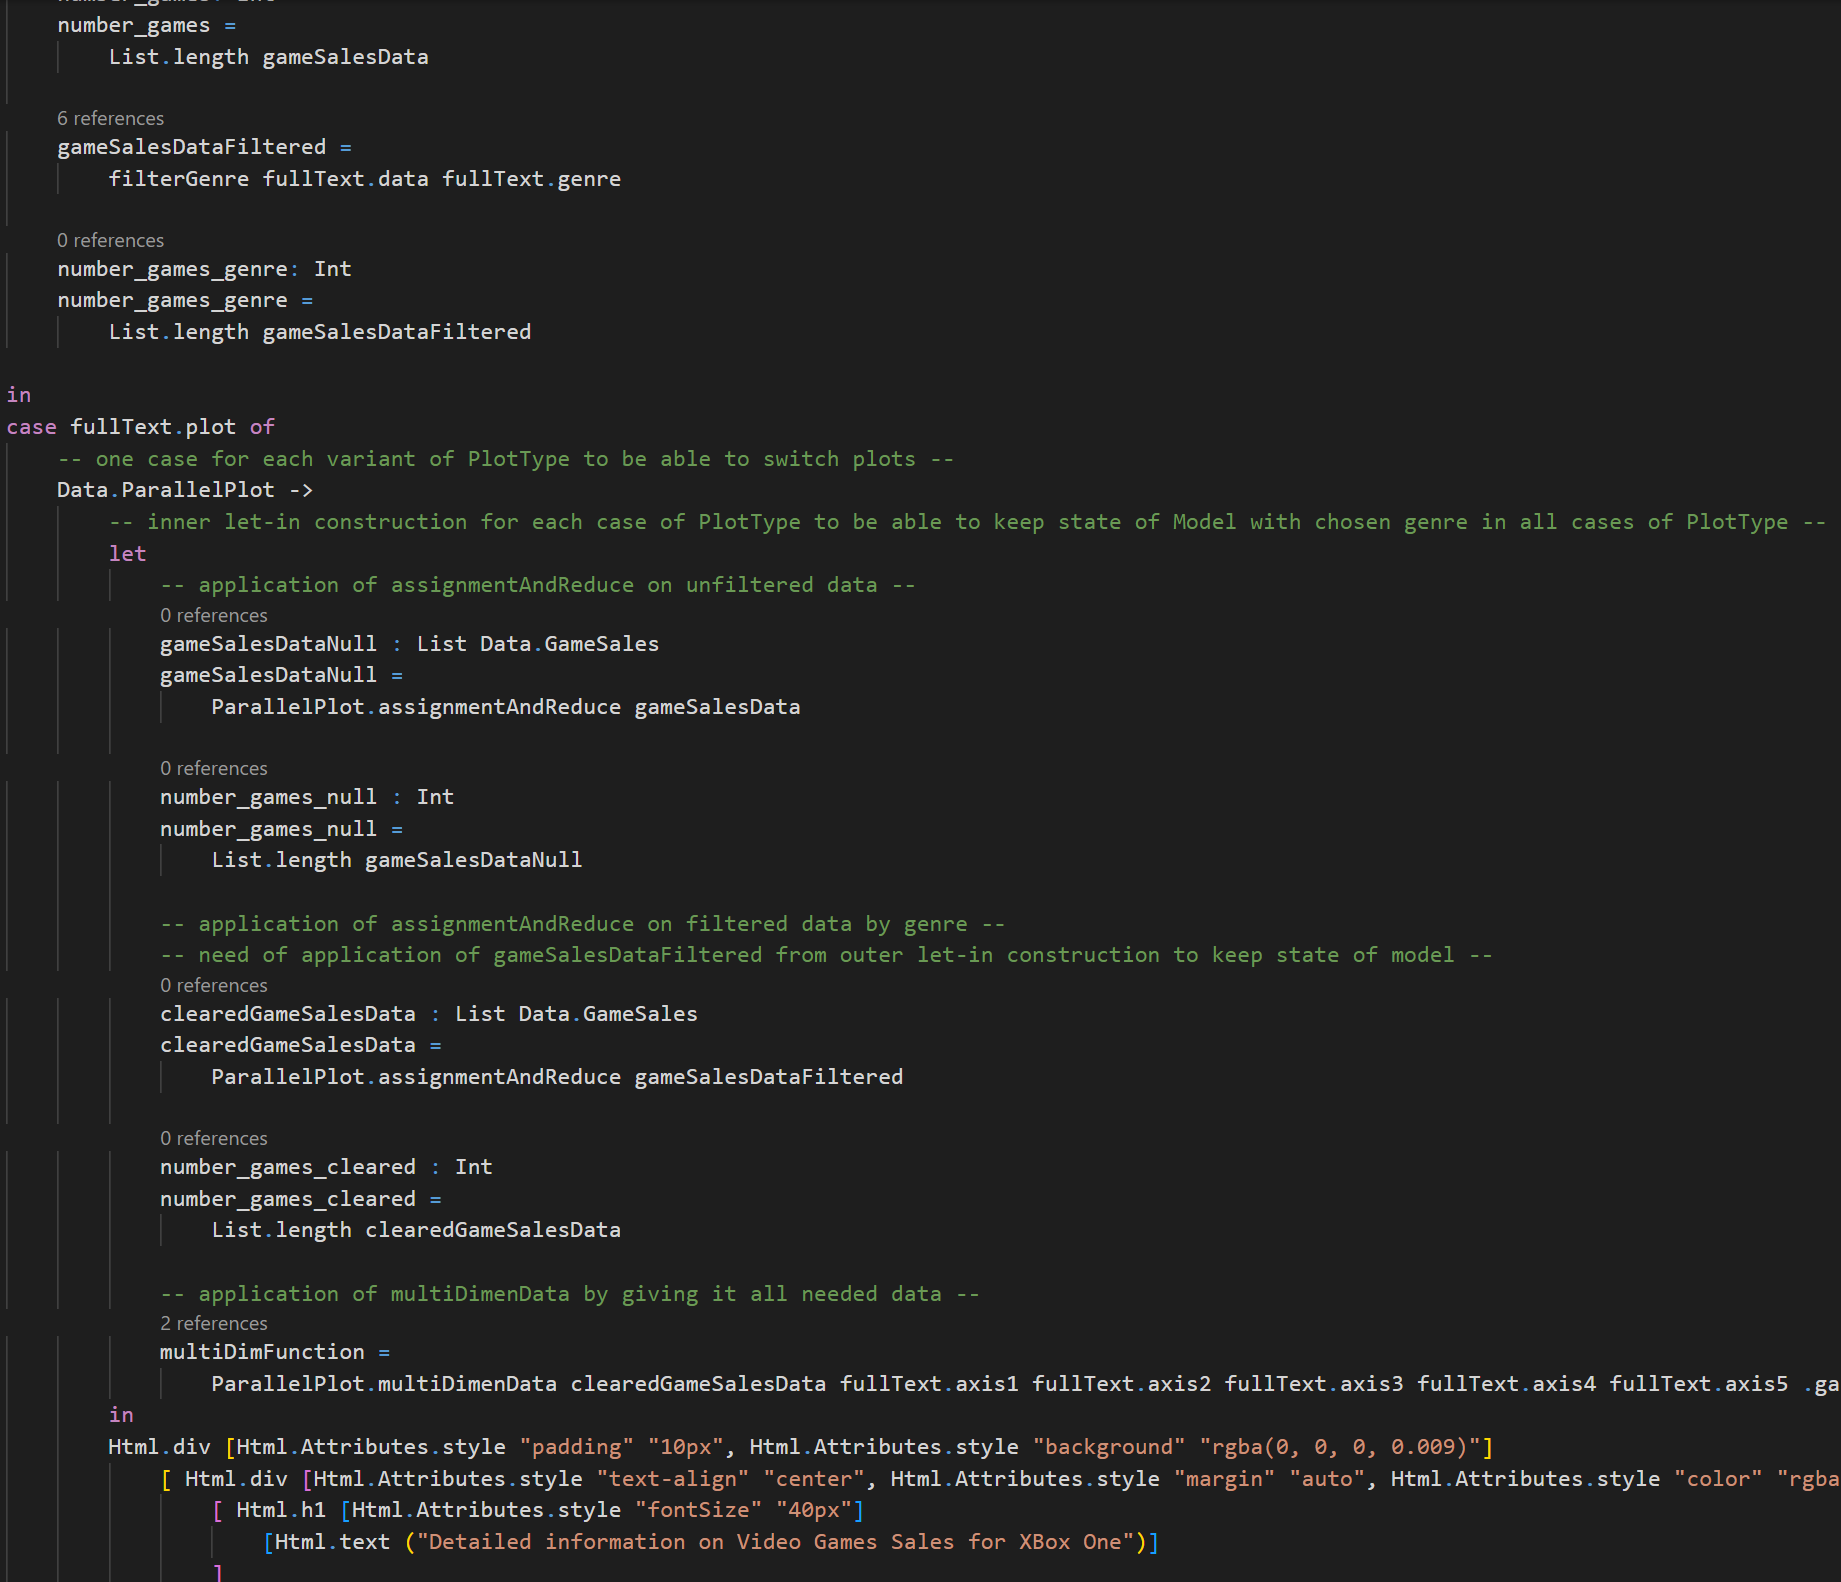
\includegraphics[width=9.5cm]{Bilder/Code_letinconstruction.png}
        \caption{Ausschnitt der verschachtelten Let-In-Konstruktion}
        \label{fig:LetIn}
\end{figure}
Je nachdem, welcher Plot mittels Button ausgewählt und das Model durch \textit{update} überschrieben wird, wird einer der drei Fälle angezeigt. 
Der Zustand des Models mit gefiltertem Genre soll bestehen bleiben, 
sodass eine Interaktion mit dem Genrebutton in einer Visualisierung zu einer Änderung der anderen führt.
Dazu dient einerseits die Variantendefinition der Plots im \textit{in}-Teil der äußeren \textit{let-in}-Ebenenkonstruktion 
sowie jeweils eine weitere \textit{let-in}-Konstruktion in den einzelnen Falldefinitionen.
Sie befinden sich auf zweiter innerer Ebene, sodass die in der äußeren Konstruktion berechneten Zustände auch hier gelten 
und bei einem Plotwechsel übernommen werden. 
In den lokalen Funktionen der inneren Konstruktion der Plots muss dazu die lokale \textit{gameSalesDataFiltered} der äußeren Ebene angewandt werden. 
Würde statt in der übergeordneten Ebene in jeder der inneren Ebenen für jeden Plot der Genrefilter neu definiert und lokal angewandt werden, 
könnten der Zustand des Models nicht übernommen werden und eine Änderung des einen würde keine Änderung des anderen Plots herbeiführen.

Der erste Case behandelt den ParallelPlot, wobei lokal die \textit{assignmentAndReduce}-Funktion auf die gesamten Daten 
sowie auf die in der äußeren Ebene nach Genre gefilterten Daten angewandt wird.
\textit{multiDimenData} wird in \textit{multiDimFunction} durch Übergabe der entsprechenden bereinigten und gefilterten Daten genutzt. 
Im \textit{in}-Teil der inneren Ebene wird die Struktur und das Design der Seite in einer wenig ablenkenden Auswahl und Abstufung zweier 
schon in den Plots vorkommenden Grüntöne sowie Ränder festgelegt.
Neben Texten werden hier auch die Buttons als Dropdown-Menü zum Wechsel des Plots, 
zur Änderung des Genrefilters sowie der Anpassung der Achsen eingefügt.
Die gewählten Einstellungen und verbleibenden Videospiele werden transparent angezeigt.
Genanntes gleicht sich in allen Plotvarianten und unterscheidet sich lediglich inhaltlich.
Schließlich werden dem \textit{scatterplotParallel} das \textit{cssParallel}, zwei Konstanten für die Höhe und die Aspect Ratio 
und die zuvor lokal berechnete \textit{multiDimFunction} übergeben.
Abschließend folgt ein Text mit Link zur TreeHierarchy in einem neuen Tab.

Im zweiten Case, dem Scatterplot, wird die Anwendung von Filter und Mapping ähnlich wie zuvor vorgenommen.
Durch die lokalen Funktionen \textit{valuesX} und \textit{valuesY} werden dem \textit{regionFilter} die nach Genre gefilterten Daten 
als Liste von GameSales und die RegionTypes der x- und y-Achse übergeben und zur Interaktion mit freier Achsenbelegung angewandt.
Im \textit{in}-Teil dieser Plotvariante werden dem \textit{scatterplot} der \textit{cssPoint}, 
die zuvor berechneten \textit{gameSalesDataCleared} sowie die \textit{valuesX} und \textit{valuesY} übergeben.
Zur Beschriftung der Achsen werden diese nach Umrechnung zu Strings hinzugefügt.

Durch die Implementierung des Baumdiagramms in \textit{TreeHierarchy.elm}, 
muss für diese Plotvariante nur die HTML-Anzeige mit Link zum Plot definiert werden.

Durch die zuvor in getrennten Anwendungen implementierten Visualisierungen war ein grundlegendes Zusammenfügen dieser 
durch stückweises Kopieren unkompliziert umsetzbar.
Die Erstellung einer einheitlichen \textit{update}-Funktion stellte sich durch die Menge an Interaktionen als zeitlich aufwendig heraus.
Schwierig war die finale Implementierung der Dropdown-Menüs für den ParallelPlot, da die Buttons zunächst je einzeln vorlagen. 
Durch Nachdenken und Ausprobieren mit \textit{multiDimenData} und verschiedenen Konvertierungsfunktionen konnten sie jedoch wie gewünscht realisiert werden.
Zur Überprüfung musste zeitaufwendig das \textit{update} immer neu angepasst werden.
Beide Plots wurden zuerst, konträr zum Gewünschten, als untereinander auf einer Seite stehend implementiert, 
sodass ohne Plot-Selektor nur eine \textit{let-in}-Konstruktion zur gleichzeitigen Filterung nötig war.
Nach schrittweisem Hinzufügen der Auswahl des Plots und allen zugehörigen Codeteilen wurde durch Ausprobieren entdeckt, 
dass eine Übernahme des Modelzustands durch Schachtelung der \textit{let-in}-Konstruktionen 
und der Anwendung des Plotvariantenwechsels mittels \textit{PlotType} möglich ist. 
Der Überblick über diese sowie außen und innen definierte lokale Funktionen gestaltete sich als kompliziert.

\section{Anwendungsfälle}
Im folgenden Kapitel wird ein möglicher Anwendungsfall der implementierten Visualisierungen präsentiert.
Dabei präsentiert ein mittlerer Manager des Publishers \textit{505 Games} die Visualisierungen zur Vorstellung der Erkenntnisse dem oberen Management sowie den Stakeholdern des Unternehmens, um weiter analysierend eine fundierte Investitionsentscheidung zu treffen. 
Es sollen Indikatoren für potenzielle Investitionen in neue Videospiele bzw. Fortsetzungen vorhandener Titel eines Genres gefunden werden, die zu einer Entscheidung zur Inauftraggabe detaillierter Marktstudien in den identifizierten Genres und potenziell zu fokussierenden Regionen führen.

\subsection{Anwendung Visualisierung Eins}
Wie in allen Visualisierungen übereinstimmend enworfen, wird auch im expliziten Baumdiagramm mittels teils minimaler farblicher Unterschiede der einzelnen Websitebereiche und der Abgrenzung der Container durch Umrandungen 
das Auge der Betrachter schnell und indirekt auf die wichtigen Steuerungselemente sowie die eigentliche Visualisierung gelenkt.
Sitzt eine Person mit Farbsehschwäche unter den Präsentationsteilnehmern, so ist dies durch Abstufungen der Grüntöne und des Kontrastes auf der Website und in den Visualisierungen unproblematisch. 

Der erste Ausschnitt des Baumdiagramms gewährt den Teilnehmern einen Überblick über alle Publisher sowie die eigene Position im Baum.
Im zweiten, detaillierteren Ausschnitt wird den Managern und Stakeholdern dargestellt, welche Genres sie mit \textit{505 Games} bedienen und welche ihrer Spiele in welches Genre passen.
\begin{figure}[h]
        \centering
        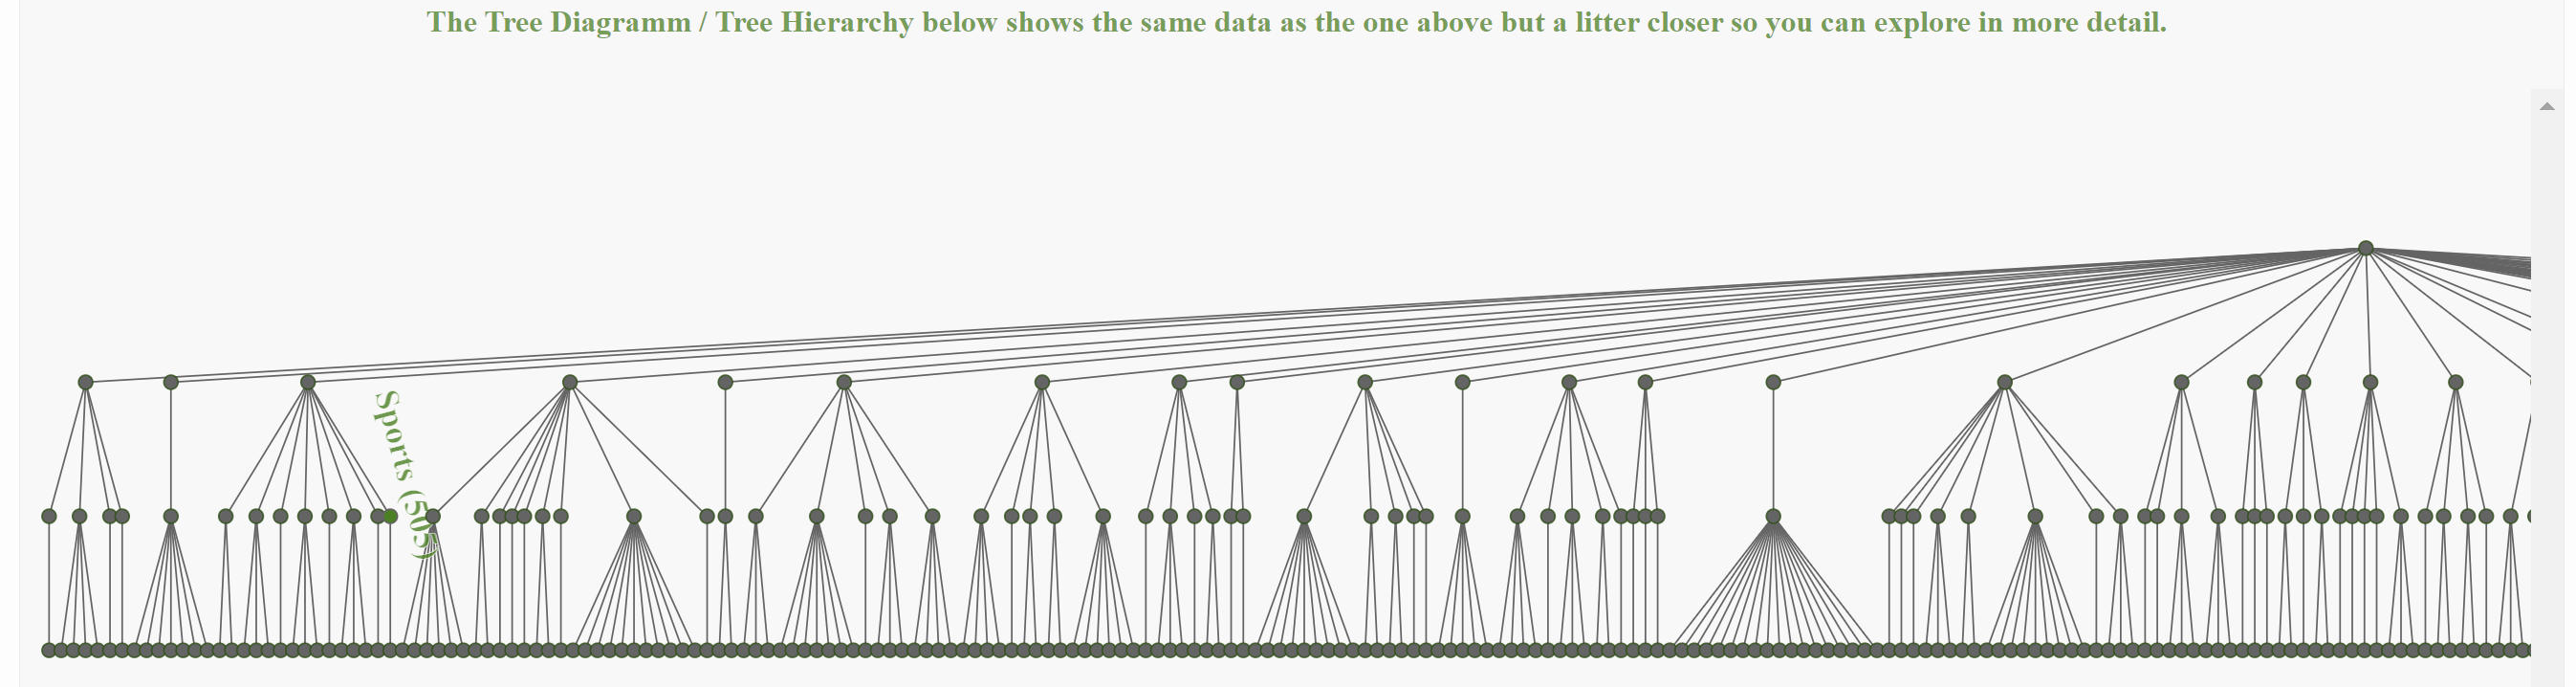
\includegraphics[height=3.5cm]{Bilder/TreeHierarchy_505Sports.png}
        \caption{Explizites Baumdiagramm mit Einblendung des Genres \textit{Sports}}
        \label{fig:TreeHierarchySports}
\end{figure}
Durch die einfache Baumstruktur ist schnell erkennbar, dass sie fünfzehn Videospiele in acht Genres anbieten, wobei \textit{Adventure}, \textit{Racing} und \textit{Shooter} die meisten Spiele aufweisen.
Dank Einblendung der Titel und Genres beim Hovern über die sich grün färbenden Knoten in beiden Diagrammen sowie das Scrollen im zweiten Diagramm sind konkrete Ein- und Überblicke effektiv möglich. 
Die Genres \textit{Action} und \textit{Sports} werden aufgrund der bisher eher geringen Ausprägung im eigenen Unternehmen näher betrachtet. 

Durch die hohe Zahl der anbietenden Publishern ergibt sich vor allem Konkurrenz im Genre \textit{Action}, wodurch eine Sicht auf mögliche Abhängigkeiten zwischen den Regionen der Welt und die entsprechend beste Positionierung im Markt wichtig ist.
Schnell erkennbar durch Struktur und Positionierung der Knoten, zeigen sich vor allem \textit{Activision}, \textit{Capcom}, \textit{Ubisoft} und \textit{Warner Bros.} durch ein hohes Spieleangebot als stärkste Konkurrenz. 
Das große Angebot in dem Genre kann Potenzial durch möglicherweise viele Käufer bieten.
\textit{Sports} hat weniger Konkurrenz, allerdings wird es durch Publisher wie \textit{EA Sports} und \textit{2K Sports} dominiert.
Aufgrunddessen entschied der Präsentator im Vorfeld, nachfolgend \textit{Action} und \textit{Sports} zu fokussieren.

Auch ein implizites Baumdiagramm hätte dem Informationsbedarf genügt. 
Aufwand und Schwierigkeit der Implementierung wären im Vergleich leicht erhöht, das Verständnis bei den potenziell ungeschulten Betrachtern wie bspw. Stakeholdern, gerade in kurzen Momenten einer Präsentation, aber gemindert. 
Hyperbolische Baumdarstellungen wären möglich, würden gut verstanden, zögen aber erhöhten Aufwand und Schwierigkeiten der Implementierung mit sich. 

\subsection{Anwendung Visualisierung Zwei}
Mit der Visualisierung des Parallelen Koordinaten Plots präsentiert der mittlere Manager einen detaillierteren Blick auf die Verkaufszahlen der Videospiele eines Genres in allen Regionen der Welt.
Es finden sich Erklärungen zu Einheiten und Darstellungsweisen auf der Website.

Das festgelegte Genre \textit{Action} wird ausgewählt, sodass die Visualisierung mit voreingestellten Achsenbelegungen 
und den gefilterten Videospielen betrachtet werden kann. 
Schnell fällt Japan auf, das viele Titel mit Verkaufszahlen von null aufweist. 
Weiterhin scheint es durch im Vergleich besser oder schlechter verkaufte Spiele keine Beziehungen zwischen den Regionen mit Japan zu geben.
Um Zusammenhänge zwischen den anderen Regionen besser erkennen zu können, wird die letzte Achse unverändert mit Japan belegt.
\begin{figure}[h]
        \centering
        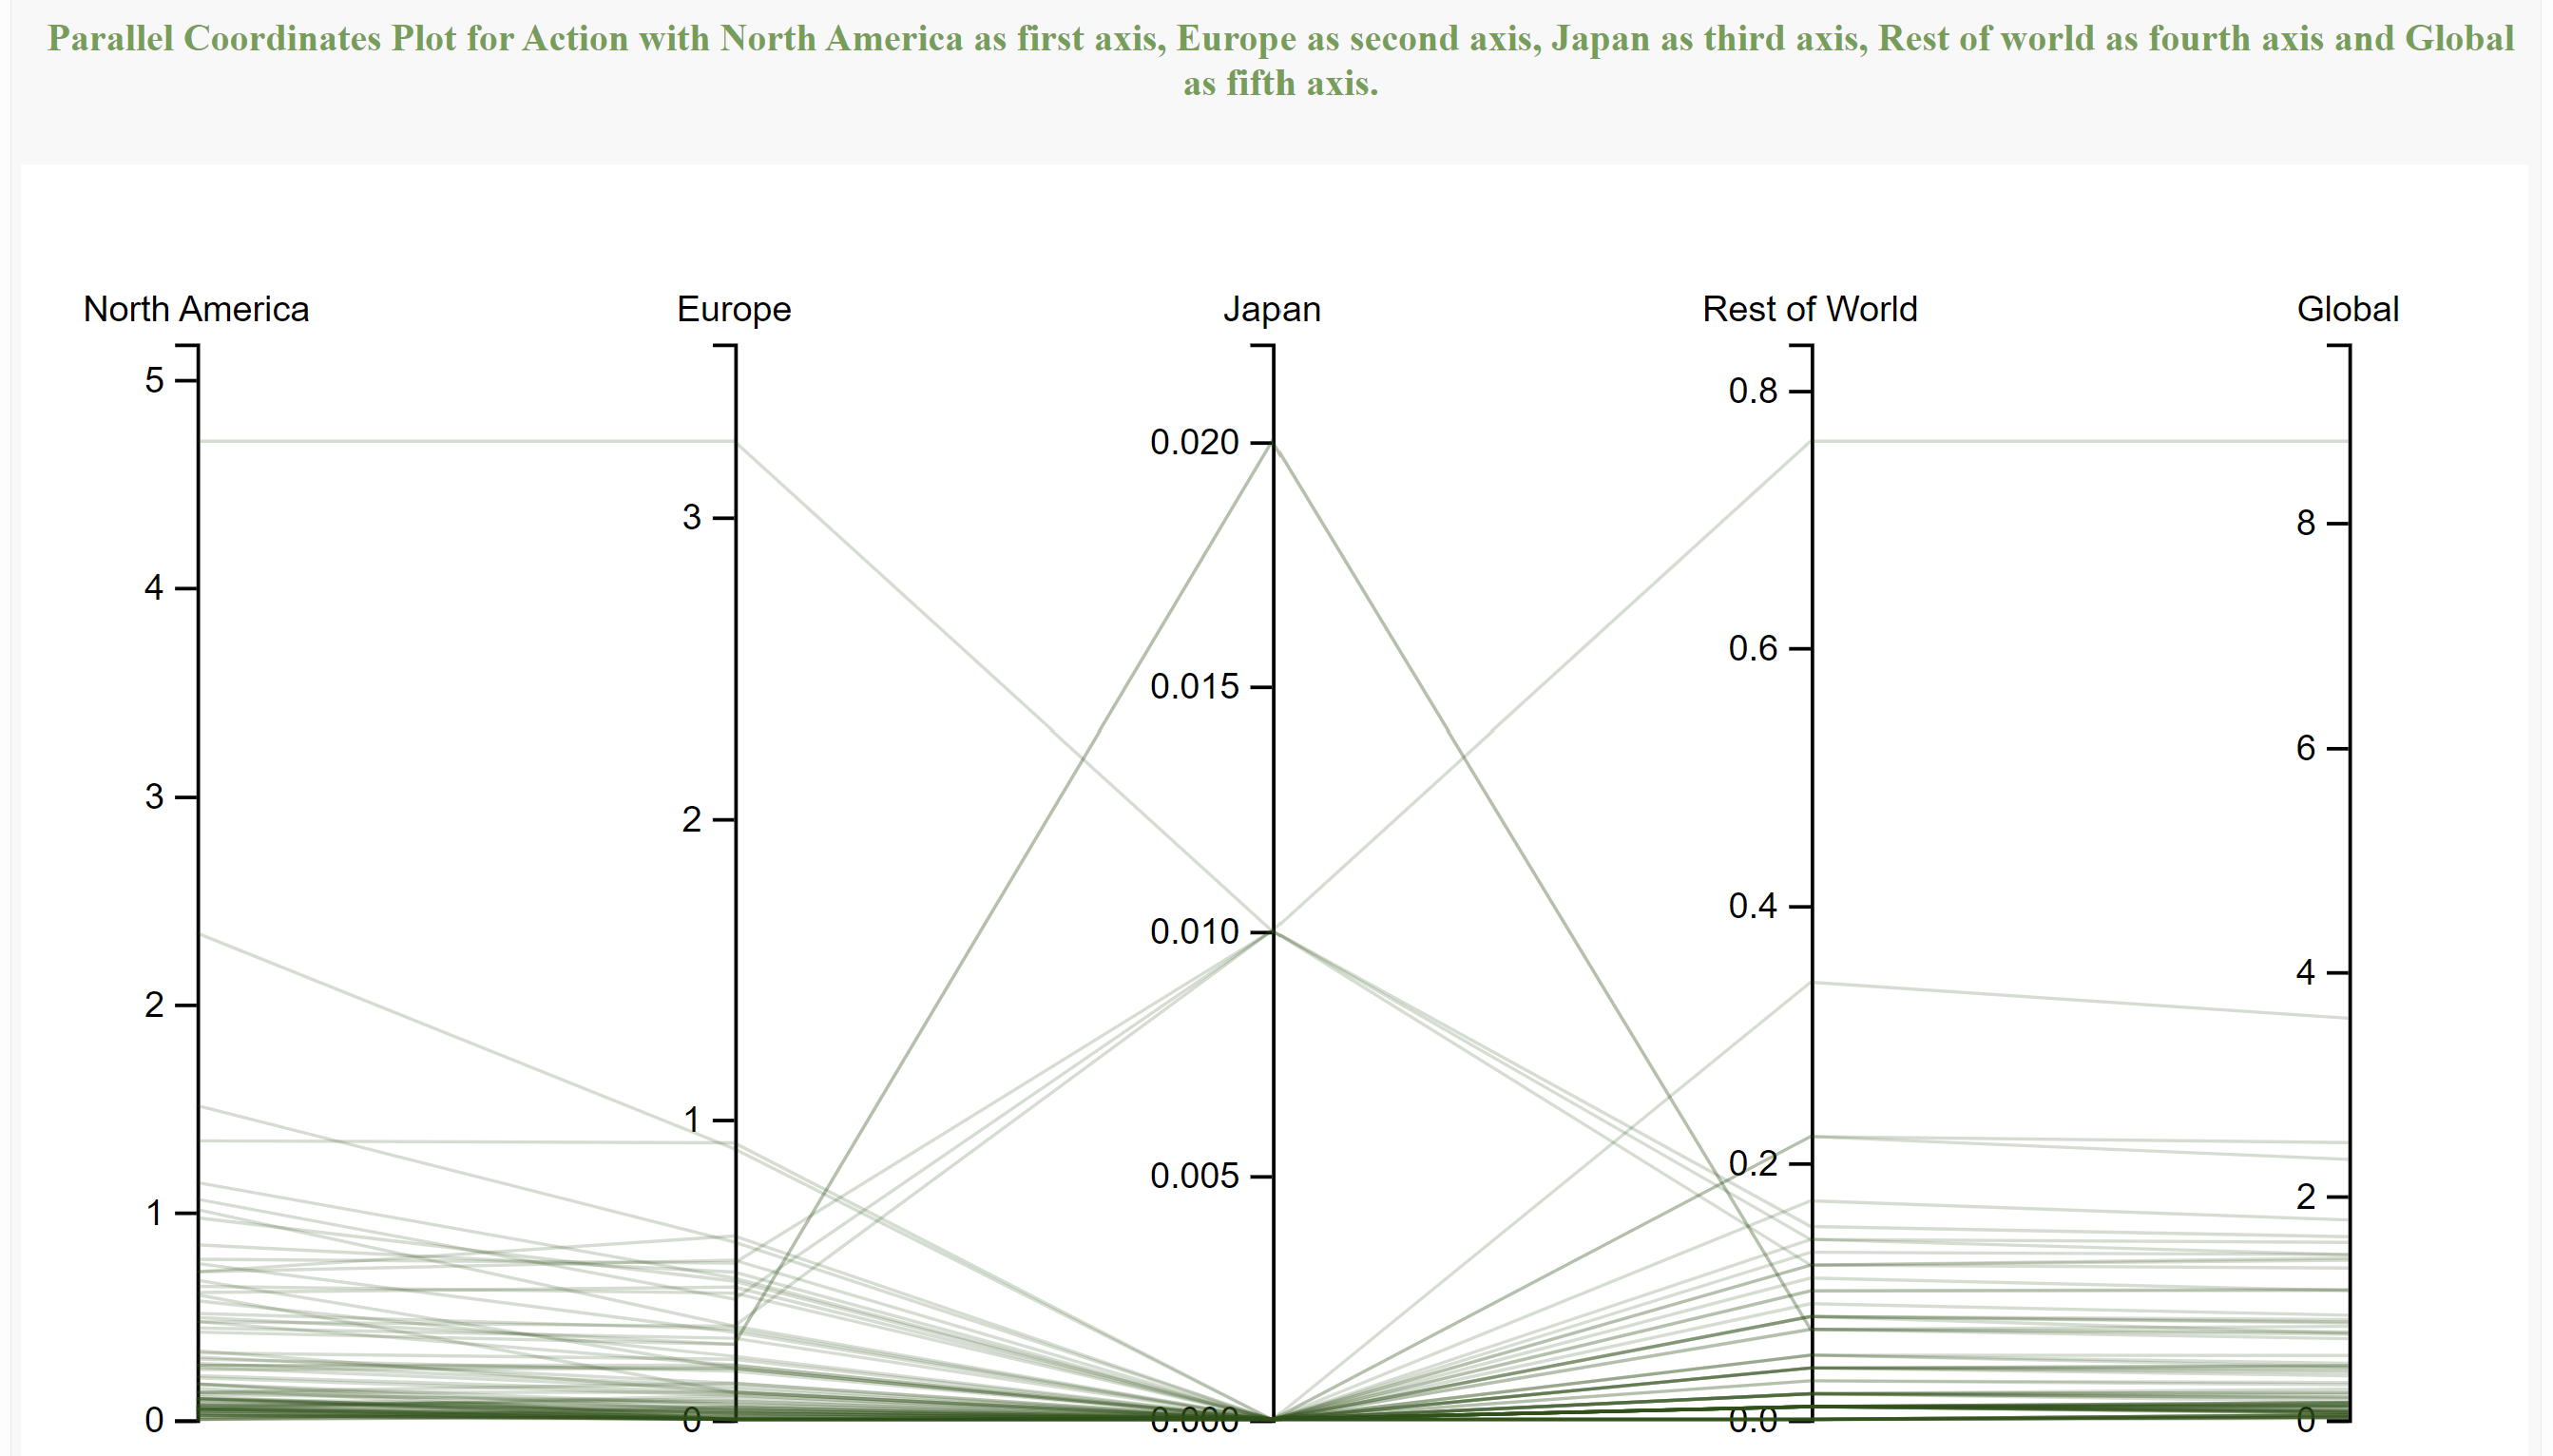
\includegraphics[height=4.5cm]{Bilder/ParallelPlot_Action.png}
        \caption{Parallele Koordinaten im Genre \textit{Action}}
        \label{fig:ParallelPlotAction}
\end{figure}
Es lässt sich immer dasselbe Muster erkennen, bestätigt und verdeutlicht durch diverse Kombinationen der Achsenbelegung und der Röntgenstrahlentechnik.
Einerseits befindet sich der Großteil der Videospiele in allen Regionen im unteren Drittel der Verkaufszahlen, was durch die Überlappungen der Datenpunkte und damit kräftigeren Grüntöne gut erkennbar ist.
Andererseits scheint es Abhängigkeiten zwischen allen Regionen außer Japan zu geben, erkenntlich durch die konstant waagerecht verlaufenden Datenpunkte.
\textit{Grand Theft Auto V} von \textit{Rockstar Games} fällt als Ausreißer auf. 

Durch die positive Korrelation scheint eine möglichst universelle Aufstellung und Nutzung der Synergieeffekte durch Abhängigkeiten nützlich.
Positive Korrelationen werden zudem als erstrebenswert für global agierende Unternehmen gedeutet, was das Genre \textit{Action} vorteilhafter für eine weitere Investition macht.
Gleichzeitig weist eine Clusterbildung im unteren Drittel der Verkaufszahlen aller Regionen auf starke Konkurrenz oder mögliche Sättigung im Genre hin. 
Sollte die Entscheidung zu weiteren Marktstudien in diesem Genre getroffen werden, 
müsste anhand weiterer Einflussparameter unter anderem der Grund für die hohen Verkaufszahlen des Ausreißers geprüft sowie die Sättigung des der Märkte und Einflussfaktoren der Verkaufszahlen der weiteren Spiele analysiert werden.
Aufgrund der unkomplizierten Erkenntnisse aus dieser Visualisierung ist eine Überprüfung im Scatterplot nicht zwingend nötig.

Im Genre \textit{Sports} gibt es keine Ausreißer über alle Regionen hinweg. Auch die Verkaufszahlen verteilen sich stärker über die Skalen. 
Japan mit in nahezu allen Titeln erkennbaren Verkaufszahlen von null bleibt bestehen und wird aus weiteren Analysen ausgenommen.
Im unteren Bild erkennbar ist jedoch die leichte Bildung verschiedener Cluster, die sich auch mit unterschiedlichen Achsenbelegungen bestätigt.
\begin{figure}[h]
        \centering
        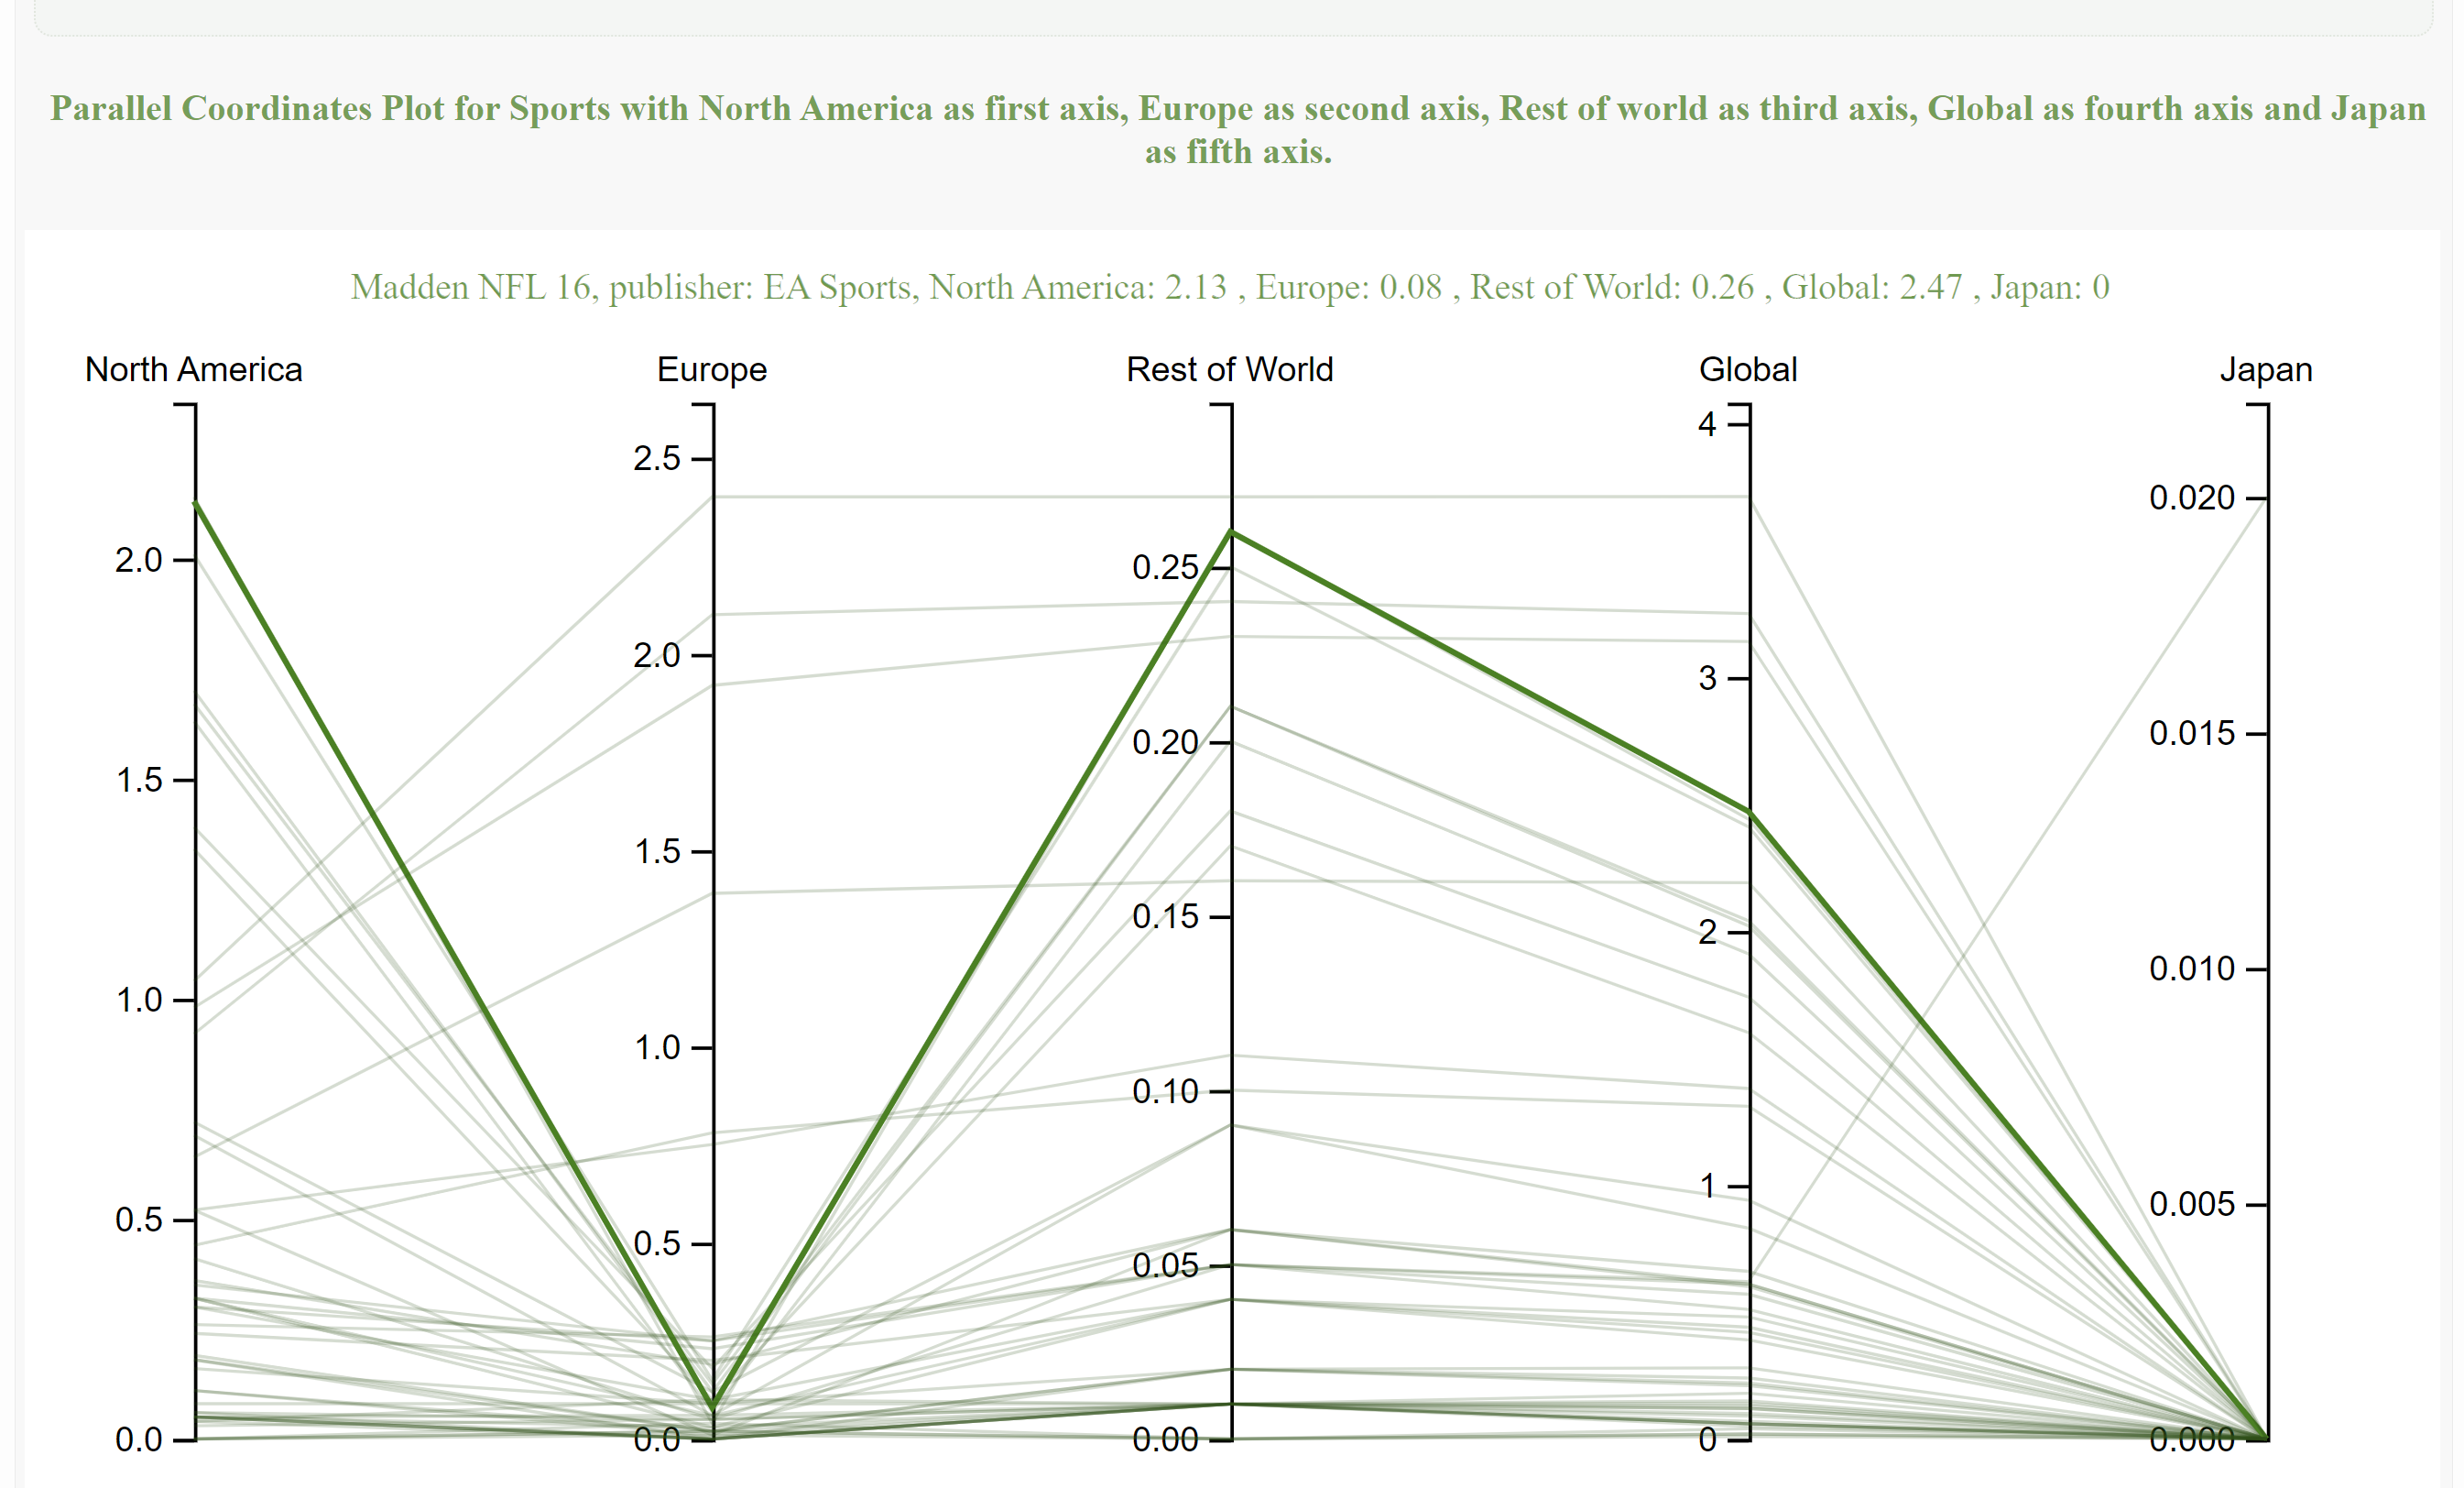
\includegraphics[height=5.5cm]{Bilder/ParallelPlot_Sports.png}
        \caption{Parallele Koordinaten im Genre \textit{Sports}}
        \label{fig:ParallelPlotSports}
\end{figure}
Es scheint eine Gruppe Spieletitel zu geben, die in Nordamerika und dem Rest der Welt gut verkauft werden konnten, global und vor allem in Europa deutlich schlechter.
Weiterhin deutet sich, wenn auch nur sehr schwach sichtbar, ein Cluster an, in dem Spiele überall gut verkauft werden, in Nordamerika im Vergleich jedoch nicht.
Die restlichen Spiele bilden ein weiteres Cluster am unteren Skalenrand mit durchgängig positiven Abhängigkeiten. 
Da sich diese Cluster besonders durch Unterschiede zwischen den Verkaufszahlen in Europa und Nordamerika unterteilen, werden diese im Scatterplot näher betrachtet. 

Der Vergleich mehrerer Dimensionen resp. mehrerer Attribute eines Videospiels wäre auch durch Icontechniken möglich. 
Diese Methode ist jedoch durch die Anzahl der zu erstellenden Icons und Kodierung der Daten auf diese aufwendiger zu erstellen und die Analyse
gestaltet sich durch möglicherweise zu wenig vorhandene Datenpunkte zur Musterbildung und einer erschwerten Erkennung konkreter Zusammenhängen zwischen allen Regionen kompliziert.

\subsection{Anwendung Visualisierung Drei}
In seiner Präsentation wählt der mittlere Manager nun den Scatterplot im Drop-Down-Menü aus.
Die zuvor getroffene Auswahl des Genres, zuletzt \textit{Sports}, bleibt bestehen und 
er belegt Achsen in einem weiteren Drop-Down-Menü mit \textit{North America} und \textit{Europe}.

Die zuvor erkannten Cluster in den Verkaufszahlen im Vergleich von Nordamerika zu Europa verdeutlichen sich. 
Manager oder Stakeholder, die die vorherige Visualisierung möglicherweise weniger gut nachvollziehen konnten, verstehen nun zumindest deutlich die Abhängigkeiten zwischen zwei visualisierten Dimensionen. 
Im unten abgebildeten Scatterplot ist deutlich ein positiv korreliertes Cluster sichtbar. 
Im zweiten zuvor entdeckten Cluster lässt sich auch bei Achsentausch keine Korrelation zwischen den Regionen finden, kennzeichnet duch die rein waagerechte bzw. senkrechte Verteilung.
Einzig das dritte Cluster lässt sich nicht direkt bestätigen, deutet sich aber durch einen Punkthaufen nahe des Ursprungs an.
\begin{figure}[h]
        \centering
        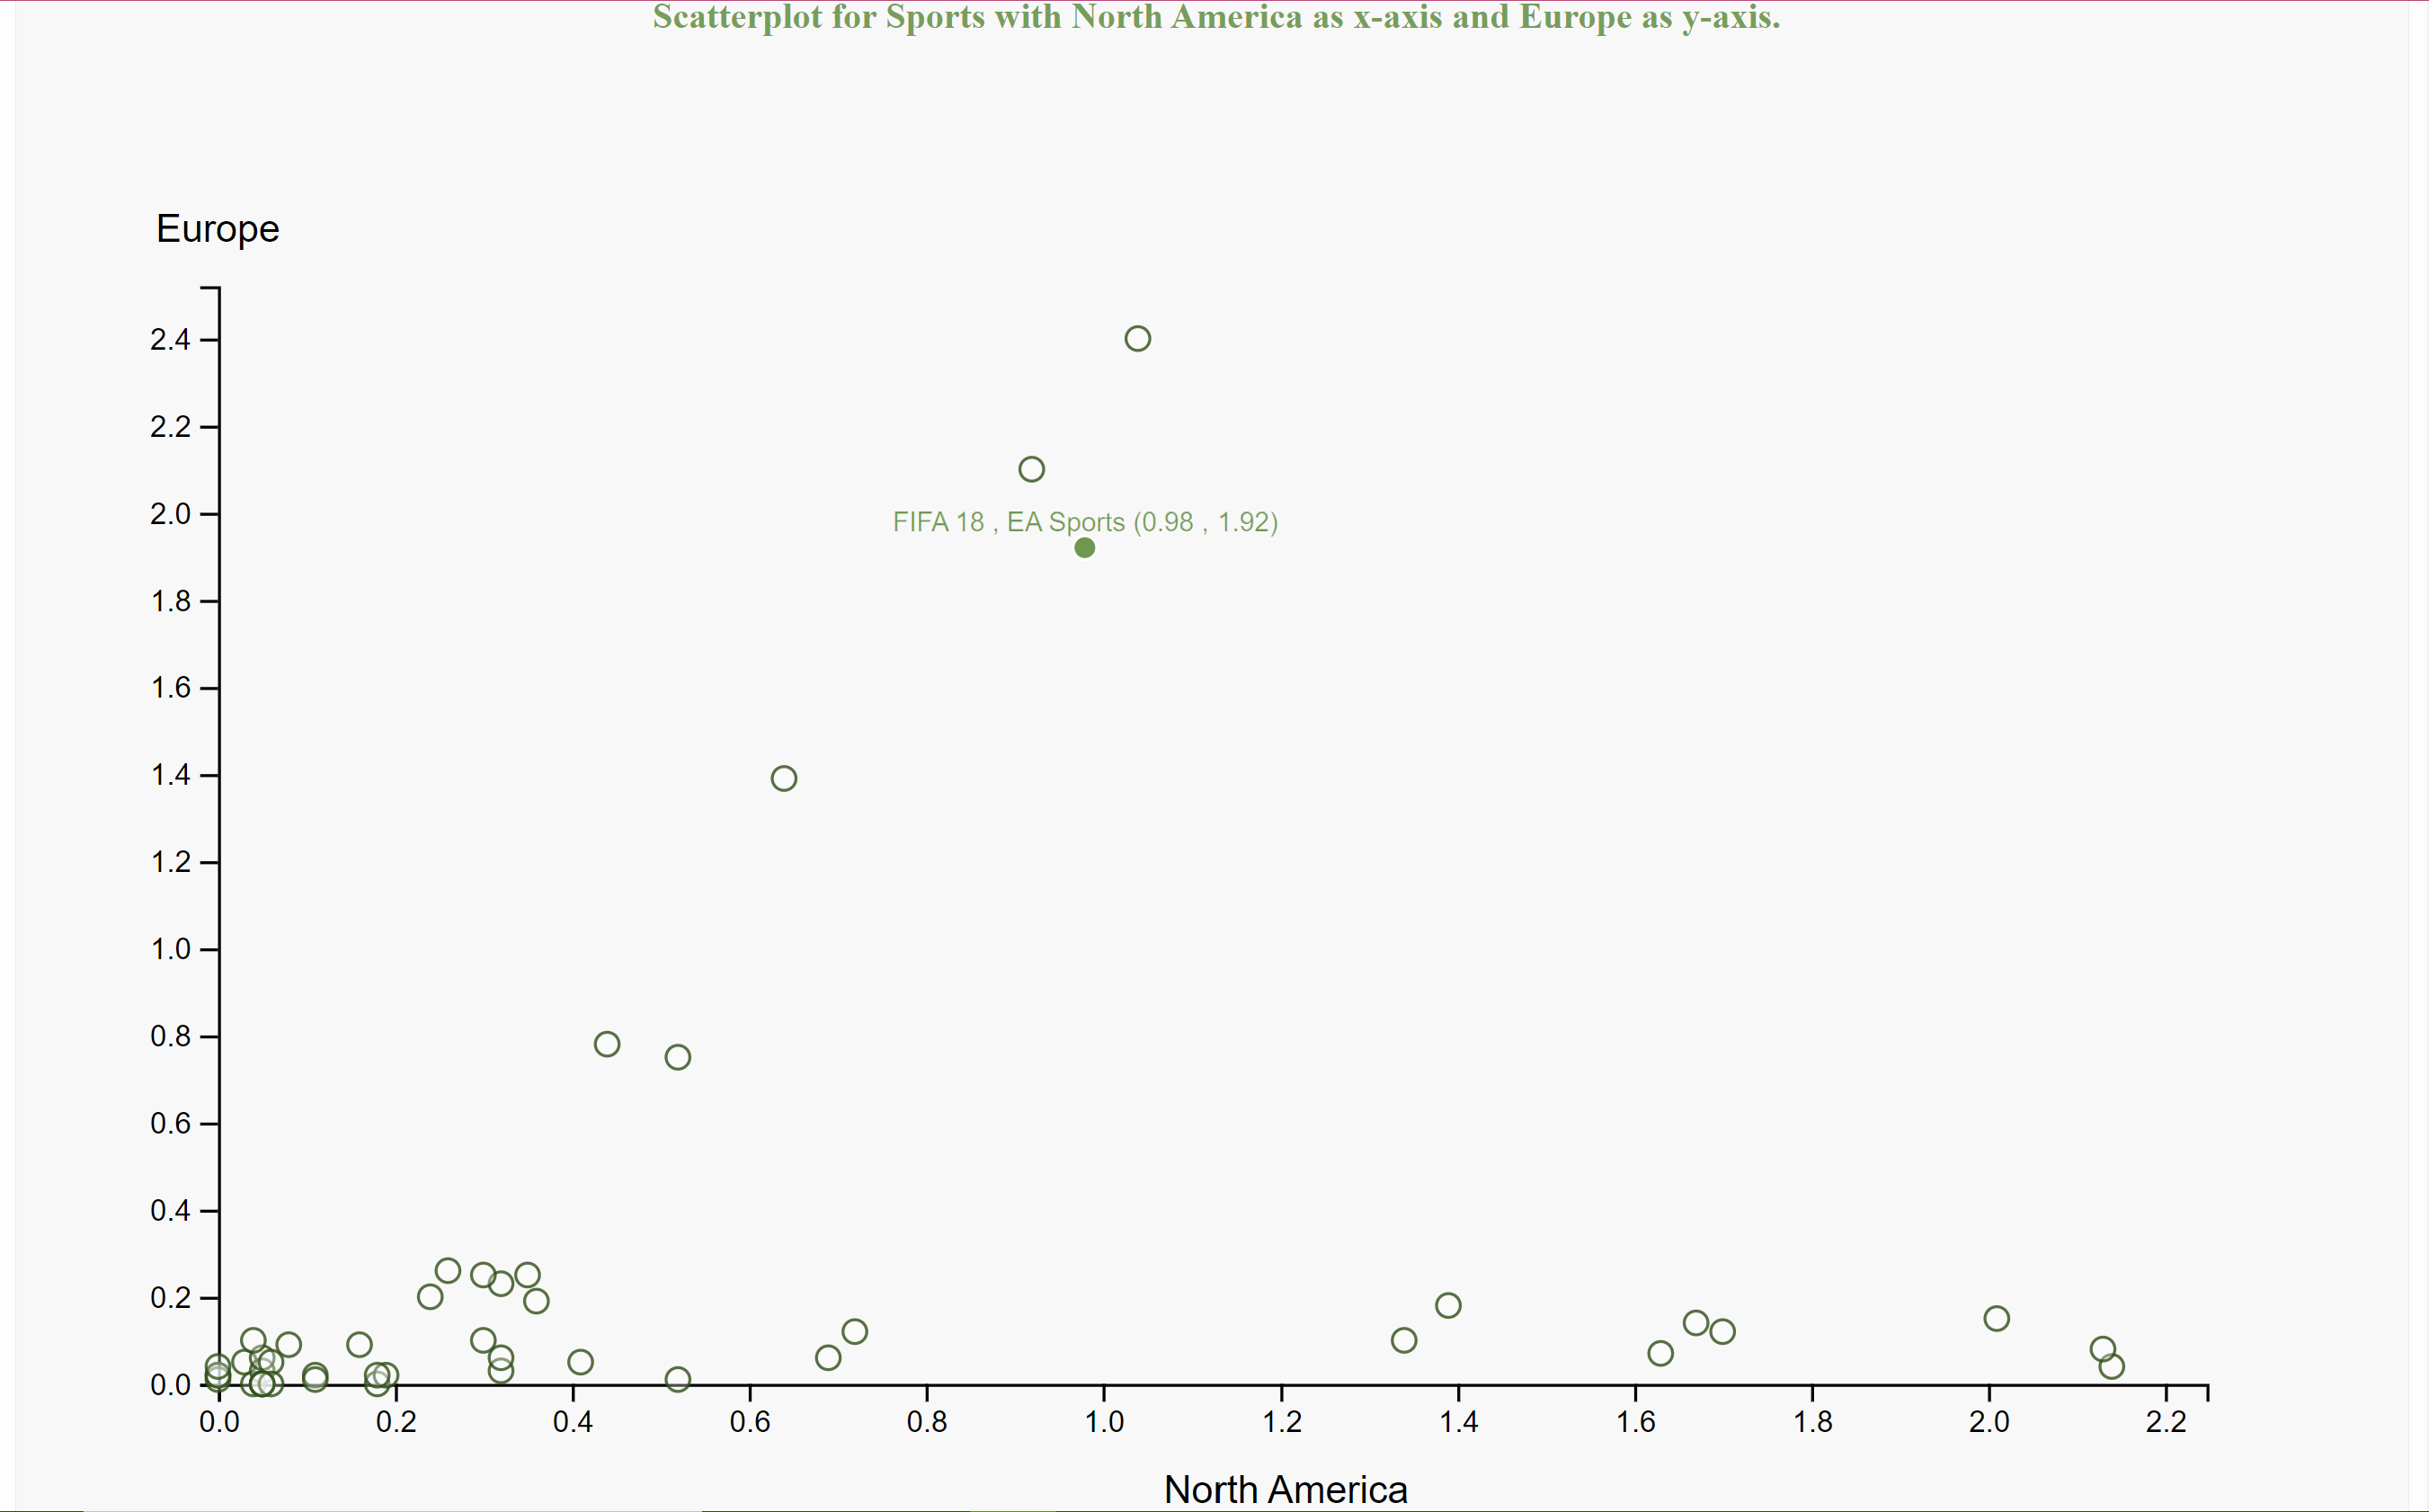
\includegraphics[height=4.8cm]{Bilder/Scatterplot_Sports.png}
        \caption{Scatterplot im Genre \textit{Sports}}
        \label{fig:ScatterplotSports}
\end{figure}
Die Erkenntnisse aus der zweiten Visualisierung werden bestätigt. 
Sportvideospiele des ersten Clusters, die in Nordamerika gut verkauft wurden, hatten auch in Europa einen guten Absatz und durch Achsentausch erkennbar auch umgekehrt.
Dort zeigt ein flacherer Anstieg zeigt auch, dass gut in Europa verkaufte Spiele in Nordamerika weniger gut verkauft wurden. 
Sehr gute Verkaufszahlen der anderen Gruppe in Nordamerika haben keinen Einfluss auf die Verkäufe in Europa, schlechte Verkäufe in Europa ebenso nicht auf die nordamerikanischen. 
Die konkreten Details der Datenpunkte zeigen, dass jene Cluster mutmaßlich in der unterschiedlichen Popularität der Sportarten in den Regionen begründet sind. 
Fußball scheint auch in Nordamerika beliebt, Football in Europa weniger.

Eine sinnvolle Alternative zu Scatterplots ist nicht gegeben, 
da sie die leichteste, deutlichste Darstellung von Beziehungen zweier Attribute eines Datenpunktes liefern. 

Abschließend kann sich das obere Management und wichtigsten Stakeholder von \textit{505 Games}
zu einer Investition in eine (kosten-) intensive Marktstudie zur Beurteilung weiterer Einflüsse im Genre \textit{Sports} entscheiden. 
Die eigene Präsenz dort ist ausbaufähig, es gibt weniger und in der Masse weniger starke Konkurrenz als bei \textit{Action} sowie keine extremen Ausreißer.
Zwar verzichtet man auf Nutzung der positiven Korrelationen zwischen allen Regionen, kann aber durch Fokussierung auf beliebte Sportarten des europäischen Marktes diese Abhängigkeiten, begrenzt auch in Nordamerika, nutzen.
Für einen vergleichsweise kleineren Publisher ist diese Strategie durch effizienten Einsatz von Mitteln sinnvoller.
 
\section{Verwandte Arbeiten}
Dieses Kapitel stellt zwei ähnliche Anwendungen zu Videospielverkäufen oder Verkaufsdaten im Allgemeinen im Bereich der Visual Analytics vor. 

Zuerst sei \textit{VizInteract: Rapid Data Exploration Through Multi-touch Interaction with Multi-dimensional Visualizations} von Chakraborty/Stuerzlinger genannt, 
in dem das Tool \textit{VizInterct} vorgestellt und getestet wird.\cite{Chakraborty.2021}
Es dient der Multi-Touch Interaktion, um multidimensionale Datenvisualisierung schneller und einfacher konstruieren und mit ihr interagieren zu können.
Es sind verschiedene Datenvisualisierungen implementiert, die mittels Ver- und Übereinanderschieben zu neuen Plots resultieren.
Beispielhaft sei hier das Übereinanderschieben zweier orthogonaler Histogramme zu einem Scatterplot genannt. 
Das Forschungsziel ist die Evaluation des Tools durch Beobachtung des Nutzerverhaltens bei einfachen touchbasierte Interaktionen.

Den Testnutzern wird unter anderem ein Unterdatensatz der \textit{Video Game Sales 2019} bereitgestellt, 
aus dem sie mit \textit{VizInteract} Visualisierungen erstellen und Analysefragen beantworten sollen.
Der Datensatz ähnelt dem hier verwendeten, gleicht sich jedoch nicht. 
\textit{VizInteract} ermöglicht Histogramme, Scatterplot (-matrizen), Parallele Koordinaten Plots und Sterndiagramme. 
Zwei der verwendeten Visualisierungstechniken werden auch im vorliegenden Projekt verwandt. 

Gemeinsamkeiten des vorliegenden Projektes und des Artikels liegen in der Möglichkeit, Notwendigkeit und 
Umsetzung von Interaktionen für sinnvolle Visualisierungen, bspw. mittels Filtern.
In beiden Fällen werden Scatterplots und Parallele Koordinaten eingesetzt und in den gestellten Aufgaben und 
im Anwendungsfall des Projektes ähnlich angewandt. 
Am Umfang \textit{VizInteracts} und seiner Tests zeigt sich die Wichtigkeit, die die Autoren den Visual Analytics beimessen.
Deutlich zeigt sich die Gemeinsamkeit der Nutzung der Videospielverkäufe mit einem sehr ähnlich aufgebauten Datensatz sowie den Visualisierungen.
Unterschiede ergeben sich aus den zusätzlichen Visualisierungstechniken des Tools sowie der Bedienbarkeit und Interaktion durch Komposition mittels Touch-Oberflächen. 
Unterschiedlich ist auch der Fokus auf Prüfung und Handhabung des Tools mittels Anwendungsfällen statt umgekehrt.

Als Zweites sei \textit{Intelligent Visual Analytics Queries} von Hao et al. genannt.\cite{Hao.2007}
Mithilfe des hier vorgestellten Tools \textit{Intelligent Visual Analytics Query} sollen Analysten bei der Untersuchung 
von großen multidimensionalen Datensätzen unterstützt werden.
Einsichten in komplexe Muster, Phänomene und Ausreißer sollen mit dessen Hilfe verbessert werden.
Die angestrebte Anwendung beschreibt einen Analysten, der in einer unkonkreten Datenvisualisierung einen Interessenbereich 
sowie die dazugehörigen Attribute auswählt.
Anschließend werden durch automatische analytische und visuelle Analysemethoden Charakterisiken und Beziehungen 
zu anderen Attributen und Datenpunkten identifiziert.
Der Anwendungsfall bezieht sich durch von Verkaufsanalysten gewünschte Korrelationen zwischen Produktverkäufen und Promotionen 
auf Verkaufszahlen von Produkten und Kundenkaufverhalten.

Das Tool nutzt zu Beginn eine visuelle Karte, in der zeilenweise Gruppen an Dimensionen und spaltenweise Datenintervalle gespeichert werden.
Farben kennzeichnen die Attributwerte der Datenpunkte zur Erkennung von Korrelationen und Ähnlichkeiten mehrerer Attribute.
Weiterhin wird wie in der hier vorliegenden Arbeit der Parallele Koordinaten Plot visualisiert. 
Dabei können interessante Untergruppen von Daten ausgewählt und die paarweise Korrelation der gewählten Attribute berechnet werden. 
Die Achsen werden so angeordnet, dass hochkorrelierte Attribute nah beieinander platziert sind. 
Auch Scatterplots als Scatterplot-Matrizen werden verwendet, um weiterhin multidimensionale statt zweidimensionale Daten abzubilden.

Gemeinsamkeiten liegen in der Auswahl und Anwendung der Visualisierungstechniken zum Erkennen von Mustern und Korrelationen 
in großen multidimensionalen Datensätzen zu Verkaufszahlen.
Zusätzlich wird die Nützlichkeit dieser Techniken und der Visual Analytics allgemein für die Auswertung und 
das Verständnis von Verkaufsdaten ähnlich eingeschätzt.
Die Nutzung und Bewertung der Existenz von Interaktionsmöglichkeiten in und zwischen Visualisierungen durch Filter 
deckt sich mit denen der Autorin der vorliegenden Arbeit.
Ein Unterschied befasst sich mit dem Einsatz von Scatterplots für Mehrdimensionalität.
Trotz Ähnlichkeiten der Parallen Koordinaten Plots ist die Anordnungsmöglichkeit der Achsen verschieden. 
Sie müssen bei Hao et al. zur besseren Erkennung von Mustern und Korrealtionen nicht selbst variabel ausgesucht werden, 
wenngleich diese Flexibilität auch fehlt.
Wie zuvor wird weniger die Beantwortung einer Frage aus der Anwendung heraus behandelt, als das Tool allgemein vorgestellt.

\section{Zusammenfassung und Ausblick}
In dieser Arbeit wurde mittels drei Visualisierungstechniken eine grobgranulare Marktanalyse 
der Verkaufszahlen des Videospielemarktes für die Konsole \textit{XBoxOne} durchgeführt, 
um die Zielgruppe des mittleren und oberen Managements sowie eingeschränkt der Stakeholder der Videospielverlage 
in ihren Investitionsentscheidungen zu unterstützen.
Sie erhalten ein schnelles Verständnis und Überblick über den aktuellen Videospielmarkt mit Fokus auf den Verkaufszahlen.
Zusammenhänge und Muster zwischen den Regionen in den Genres können ohne Vorwissen im Bereich der Visual Analytics abgelesen, analysiert und präsentiert werden.
So werden erste Erkenntnisse bezüglich neuer Möglichkeiten und Chancen im Markt sowie Ansatzpunkte für Strategieentscheidungen ermöglicht. 
Sie dienen als Entscheidungsunterstützung für die Beauftragung detaillierterer und teurerer Marktstudien für neue Investitionen.
 
Durch die Implementierung eines expliziten Baumdiagramms konnte eine hierarchische Übersicht über den Markt sowie die Zusammenhänge zwischen Publisher, Genre und Titel des eignen Verlagshauses und der Konkurrenz umgesetzt werden.
Mittels eines Parallelen Koordinaten Plots zur Darstellung mehrdimensionaler Daten konnten auch durch den Einsatz einer Röntgenstrahlentechnik 
Abhängigkeitsmuster in den Verkaufszahlen von Videospielen eines Genres über mehrere Dimensionen, also Regionen, hinweg erkannt werden.
Zuletzt konnten in einem klassischen Scatterplot die Erkenntnisse aus der vorherigen Visualisierung inklusive Clusterbildung, 
Ausreißern und Korrelationen zwischen zwei Regionen konkretisiert werden. 
Für ein verbessertes, komfortables und schnelles Anwendungserlebnis sowie Effektivität und Effizienz wurde die Auswahl der Genres mittels Drop-Down Menü interaktiv gestaltet 
sowie beim komfortablen Umschalten der Visualisierungen ebenso mittels Drop-Down Menü erhalten.
Aus demselben Grund wurde ein Beibehalten der flexiblen, individuellen Achsenauswahl für den Parallelen Koordinaten Plot sowie den Scatterplot integriert.

Eine sinnvolle Erweiterung ist der Einbezug von (Nutzer-) Kritiken und deren Auswirkungen auf die Verkaufszahlen 
sowie die Analysen von Korrelationen nicht öffentlich zugänglicher Daten zu Entwicklungskosten und Umsätzen pro Spiel.
Dies ist jedoch Teil der angesprochenen weiterführenden Marktstudien.
Interessant ist eine weitere Unterteilung der Region \textit{Rest of World}, die unter anderem Afrika, Asien und Südamerika enthält.
Bezüglich der Visualisierungstechniken können Verbesserungen und weitere Kopplungen von Interaktionen direkt in den Plots Sinn ergeben, 
sind jedoch im Kontext der Andwendungsaufgaben eine zusätzliche Spielerei.
Mehr Potenzial bieten Ansätze aus den \textit{verwandten Arbeiten}. 
So ist ein automatisches Anordnen der Achsen je nach Korrelationsstärke im Parallelen Koordinaten Plots nach Hao et al. interessant.\cite{Hao.2007}
Zur Verbesserung der Interaktionen auf der vielfältigen Wahl der Endgeräte ergibt eine Implementierung einer Komposition von Visualisierungen durch Zusammenschieben nach Chakraborty/Stuerzlinger Sinn.\cite{Chakraborty.2021}
Insgesamt konnten die Anforderungen an die Visualisierungen zur Lösung des Zielproblems jedoch zufriedenstellend umgesetzt werden.
\newpage
\section*{Anhang: Git-Historie}

\printbibliography

\end{document}

